\chapter{Implementação e aplicações}\label{capitulo:simulacao}

%%%%%%%%%%%%%%%%%%%%%%%%%%%%%%%%%%%%%%%
%%% INTRODUÇÃO / CONTEXTUALIZAÇÃO
%   Este sera um capitulo de aplicação. Falar brevemente de 
%   como serao feitos os testes e mais abertamente o que se 
%   quer aqui.
%%%%%%%%%%%%%%%%%%%%%%%%%%%%%%%%%%%%%%%
% * CONTEXTUALIZACAO E OBJETIVOS
%
%   Este sera um capitulo de aplicação. Falar brevemente de como serao
%   feitos os testes e mais abertamente o que se quer aqui.
%

O objetivo deste último capítulo é a aplicação da teoria apresentada. Começando pela implementação computacional, discutimos a escolha da linguagem de programação Fortran e a estrutura do programa final. Passamos então para as questões de valores iniciais, apresentando o método utilizado para condicionar as integrais primeiras.

A questão das colisões vem em seguida, pois existem outras formas computacionais de lidar com singularidades e aproximações intensas no PNCG além da inclusão de colisões perfeitamente elásticas.

Algumas questões sobre o corretor numérico apresentado na seção \ref{secao:corretor_numerico} também precisam ser discutidas, como o seu uso e seu custo de computação associado. Além disso, este envolve a resolução de um sistema de equações (para mais de uma integral primeira em consideração), então foi necessário escolher um método de resolução adequado.

Por fim, apresentamos algumas simulações de muitos corpos e com condições iniciais específicas para testar os resultados da Dinâmica de Formas enunciados na seção \ref{secao:dinamica_de_formas}.

Todas as simulações e testes realizados neste trabalho foram aplicados em um computador de mesa (não dedicado) com processador \textit{Intel Core i5 CPU 760 @ 2.80GHz} e com 16 GB de RAM.

% Como já explicitado, neste trabalho são consideradas os sistemas puramente gravitacionais e conservativos, além de pontuais, ou seja, cada corpo é um ponto individual. As simulações de grande porte utilizadas na astronomia e na cosmologia no geral consideram, no lugar de pontos de massa, funções de densidade $\rho$ e um campo gravitacional $\nabla \phi$, de modo que o potencial fica dado por uma equação de Poisson
% \begin{equation*}
%     \Delta \phi = - 4 \pi G \rho.
% \end{equation*}
% O campo é então discretizado através de métodos numéricos voltados para equações diferenciais parciais, e neste ponto é feita a integração numérica temporal. Isto é necessário por uma série de razões práticas, como a implementação de gases, galáxias e afins, indo bem além dos objetivos deste trabalho. [TALVEZ COLOCAR ISSO NA INTRODUÇÃO DO TRABALHO, E NÃO AQUI]

% Sendo assim, existe neste trabalho a necessidade de calcular direta e rapidamente expressões não-lineares com ordem quadrática, como o potencial gravitacional, sem o uso de aproximações como o algoritmo de Barnes-Hut [TALVEZ FALAR MELHOR SOBRE TAMBÉM, SÓ PRA NÃO FICAR JOGADO]. Isso levou à escolha do Fortran como linguagem de programação para as simulações, e suas particularidades serão melhor exploradas adiante.

%%%%%%%%%%%%%%%%%%%%%%%%%%%%%%%%%%%%%%%
%%% FERRAMENTAS
%   Defender a escolha do Fortran e apresentar informacoes
%   basicas: compilador, bibliotecas, etc.
%   Falar sobre a estrutura de dados, a forma de armazenamento,
%   a análise. 
%   Falar especificamente sobre a aplicacao no PNC, como a
%   paralelizacao, (SE ROLAR GPU TB), e especificadas do
%   codigo para o problema em questao.
%   Apresentar dificuldades.
%   Disponibilizar código.
%%%%%%%%%%%%%%%%%%%%%%%%%%%%%%%%%%%%%%%
% * FERRAMENTAS E CÓDIGO
%   
%   Defender a escolha do Fortran e apresentar informacoes
%   basicas: compilador, bibliotecas, etc.
%   Falar sobre a estrutura de dados, a forma de armazenamento,
%   a análise. 
%   Falar especificamente sobre a aplicacao no PNC, como a
%   paralelizacao, (SE ROLAR GPU TB), e especificadas do
%   codigo para o problema em questao.
%   Apresentar dificuldades.
%   Disponibilizar código.
\section{Ferramentas}

%%%%%%%%%%%%%%%%%%%%%%%%%%%%%%%%%%%%%
%%% ESCOLHA DA LINGUAGEM
%%%%%%%%%%%%%%%%%%%%%%%%%%%%%%%%%%%%%
\subsection{Escolha da linguagem de programação}
Como dito brevemente, a necessidade de muitas operações computacionalmente custosas com agilidade exigiu a escolha de uma linguagem de programação que fosse potente por natureza. 

Linguagens como o Python possuem excelentes bibliotecas voltadas para a computação científica, como o \textit{NumPy} e o \textit{SciPy}, além de bibliotecas de otimização de processamento como o \textit{Numba}. Porém, estas no geral são linguagens de programação denominadas \textit{interpretadas}, pois não têm seu código explicitamente compilado, o que no geral as torna mais lentas que linguagens explicitamente compiladas, como C, Java ou Fortran. 

Vale ressaltar que um código em Python que utilize corretamente as bibliotecas mencio\-nadas pode de fato ser mais rápido que um código não otimizado em alguma linguagem compilada. Ainda assim, o esforço necessário para isso é considerável, e neste trabalho foi escolhido o caminho de explorar a linguagem compilada \textit{Fortran}.

O Fortran, acrônimo de \textit{IBM Mathematical FORmula TRANslation System}, é uma linguagem de programação compilada criada na década de 1950 com o objetivo de ser aplicada em computação científica. Apesar de ser uma linguagem antiga, seu desenvolvimento continua e o Fortran se mantém sendo a principal linguagem utilizada para computação científica até hoje, presente, por exemplo, no NumPy e no SciPy \citep{2020NumPy-Array, 2020SciPy-NMeth}.

Existem diversas bibliotecas de Fortran voltadas para computação científica. Neste trabalho foram utilizadas duas delas: \textit{OpenMP} e o \textit{OpenBLAS}. A primeira é uma biblioteca para computação paralela, e será explorada com mais delalhes na subseção \ref{subsecao:paralelizacao}. 

Já o \textit{OpenBLAS} é uma biblioteca otimizada de \textit{BLAS} (\textit{Basic Linear Algebra Subprograms}) e \textit{LAPACK} (\textit{Linear Algebra Package}), dois conjuntos de subrotinas voltadas para álgebra linear numérica. A documentação de ambos pode ser encontrada, respectivamente, em \cite{OpenBLAS} e \cite{lapack}.

Vale ressaltar que existem também bibliotecas voltadas para a integração numérica, com métodos de alta ordem e otimizados. Porém, como o propósito deste trabalho também foi aprender a implementá-los manualmente, estas não foram utilizadas.

O repositório com o código desenvolvido pode ser acessado no endereço \href{https://github.com/potalej/gravidade-fortran}{https://github.com/potalej/gravidade-fortran} \citep{potalej_gravidade-fortran}.

%%%%%%%%%%%%%%%%%%%%%%%%%%%%%%%%%%%%%
%%% ESTRUTURA DO PROGRAMA
%%%%%%%%%%%%%%%%%%%%%%%%%%%%%%%%%%%%%
\subsection{Estrutura do programa}
O programa final é dividido em algumas sub-rotinas que são chamadas por um módulo central, o \verb|simulacao|. As sub-rotinas principais são:
\begin{itemize}
    \item \verb|simulacao|: Um módulo central \verb|simulacao| é utilizado como base para os dois módulos de simulação, o \verb|simulacao_vi| e o \verb|simulacao_sorteio|, para simulações com valores iniciais explícitos e simulações com sorteio de condições iniciais, respectivamente.

    \item \verb|integrador|: Um módulo pai o qual todos os integradores estendem, contendo rotinas para integração e para o cálculo de forças.

    \item \verb|mecanica|: Sub-rotinas de mecânica.

    \item \verb|correcao|: Sub-rotinas do corretor numérico.

    \item \verb|colisao|: Sub-rotinas das colisões perfeitamente elásticas.

    \item \verb|forcas|: Sub-rotinas de forças, sendo uma sequencial e uma paralelizada.

    \item \verb|condicoesIniciais|: Sub-rotinas para a geração aleatória e condicionamento de valores iniciais.

    \item \verb|arquivos| e \verb|leitura|: Sub-rotinas para a manipulação de arquivos.

    \item \verb|plot|: Sub-rotinas para exibição de trajetórias utilizando o \textit{GNUPlot}.
\end{itemize}

Todos os métodos de integração numérica implementados foram apresentados explicitamente neste trabalho no capítulo \ref{capitulo:metodos_numericos}. Os métodos disponíveis e testados até este trabalho constam na tabela \ref{tab:integradores_implementados}.
\begin{table}[]
    \centering
    \begin{tabular}{|c|c|c|c|c|}
        \hline
        \textbf{Módulo} & \textbf{Nome ou Tipo} & \textbf{Ordem} & \textbf{Estágios} & \textbf{Referência}
        \\ \hline
        \verb|euler|     & Euler Explícito & 1 & 1 & \ref{metodo:euler_explicito}
        \\ \hline
        \verb|euler_imp| & Euler Implícito & 1 & 1 & \ref{metodo:euler_implicito}
        \\ \hline
        \verb|rungekutta2| & Runge-Kutta & 2 & 2 & \ref{metodo:rk22}
        \\ \hline
        \verb|rungekutta3| & Runge-Kutta & 3 & 3 & \ref{metodo:rk33}
        \\ \hline
        \verb|rungekutta4| & Runge-Kutta & 4 & 4 & \ref{metodo:rk44}
        \\ \hline
        \verb|eulersimp| & Euler Simplético & 1 & 1 & \ref{metodo:euler_simpletico}
        \\ \hline
        \verb|verlet|    & Velocity-Verlet & 2 & 2 & \ref{metodo:velocity-verlet}
        \\ \hline
        \verb|ruth3|     & Ruth & 3 & 3 & \ref{metodo:ruth3}
        \\ \hline
        \verb|ruth4|     & Ruth & 4 & 4 & \ref{metodo:ruth4}
        \\ \hline
        \verb|rkn551|    & Runge-Kutta-Nyström & 5 & 5 & \ref{metodo:rkn551}
        \\ \hline
        \verb|rkn671|    & Runge-Kutta-Nyström & 6 & 7 & \ref{metodo:rkn671}
        \\ \hline
        \verb|svcp8s15|  & Stormer-Verlet Composto & 8 & 15 & \ref{metodo:svcp8s15}
        \\ \hline
        \verb|svcp10s35| & Stormer-Verlet Composto & 10 & 35 & \ref{metodo:svcp10s35}
        \\ \hline
    \end{tabular}
    \caption{Integradores numéricos implementados.}
    \label{tab:integradores_implementados}
\end{table}


%%%%%%%%%%%%%%%%%%%%%%%%%%%%%%%%%%%%%
%%% PRECISAO E ERROS DE PONTO FLOAT
%%%%%%%%%%%%%%%%%%%%%%%%%%%%%%%%%%%%%
\subsection{Precisão e erros de ponto flutuante}
Os computadores armazenam números como uma quantidade finita de \textit{dígitos binários}, os \textit{bits}. Isso significa que todo número inteiro é armazenado exatamente como é, e todo número real $\alpha$ é armazenado na representação de \textit{ponto flutuante}, no qual a mantissa do número é recortada para uma quantidade finita de dígitos.

Existem diversas formas de representação de ponto flutuante, mas a maioria dos processadores modernos segue o padrão internacional IEEE 754-185, no qual há diversos padrões de ponto flutuante. Os principais são os de 32 \textit{bits}, os de 64 \textit{bits} e os de 128 \textit{bits}. O \textit{float}, tipo dedicado para valores reais no Python, utiliza o padrão de 64 \textit{bits}. Já o \textit{real}, análogo do \textit{float} mas para Fortran, utiliza o de 32.

Para ver a diferença entre os tipos, podemos buscar o menor $\epsilon$ positivo tal que $1.0 + \epsilon \neq 1.0$, utilizando a \textit{aritmética de ponto flutuante}. Utilizando o Fortran, para o tipo \textit{real} padrão temos $\epsilon = 6.0 \cdot 10^{-8}$, enquanto que para o \textit{real64} temos $\epsilon = 1.1 \cdot 10^{-16}$ e para o \textit{real128} temos $\epsilon = 1.0 \cdot 10^{-34}$. Na prática, isso significa que a \textit{precisão} de cada tipo, ou seja, quantas casas decimais podem ser levado em conta ao final de um programa, é, respectivamente, $7$, $15$ e $33$.

Como o PNCG é um problema com momentos de instabilidade numérica, como quando ocorrem aproximações intensas, os resultados mais numericamente interessantes precisam ser pelo menos do tipo \textit{real64}. Tipos com mais \textit{bits} são computacionalmente custosos para cálculos, então optamos por utilizar o padrão \textit{real64}.

A figura \ref{fig:bits_energia} contém uma comparação das variações da energia total para diferentes tipos de \textit{float}. Vale observar que neste exemplo, a duração da simulação para \textit{real32}, \textit{real64} e \textit{real128} foi, respectivamente, 0.27, 0.39 e 15.62 segundos.

\begin{figure}
    \centering
    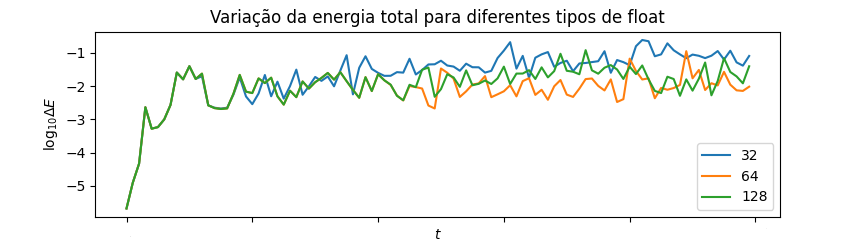
\includegraphics[width=\linewidth]{tcc//img/bits_energia.png}
    \caption{Variação da energia total no problema-modelo \ref{probmodelo:iau25} via método Ruth4 com $h=10^{-2}$ e $\epsilon=5h$ no intervalo $[0,500]$ para \textit{floats} com 32, 64 e 128 bits.}
    \label{fig:bits_energia}
\end{figure}

%%%%%%%%%%%%%%%%%%%%%%%%%%%%%%%%%%%%%
%%% PARALELIZAÇÃO
%%%%%%%%%%%%%%%%%%%%%%%%%%%%%%%%%%%%%
\subsection{Paralelização}\label{subsecao:paralelizacao}
Como mencionado anteriormente, foi utilizada uma biblioteca de Fortran para computação paralela, a \textit{OpenMP} (\textit{Open Multi-Processing}). Enquanto um código serial realiza uma operação por vez, um código paralelo é capaz de realizar mais de um cálculo ao mesmo tempo, como na figura \ref{fig:computacao_serial_paralela}. No caso do PCNG, existem algumas possibilidades para a aplicação: o cálculo do potencial e das forças, o cálculo da matriz normal utilizada no corretor numérico (ver equação (\ref{eq:corretor_matriz_normal})) e na detecção de colisões.

\begin{figure}[H]
    \centering
    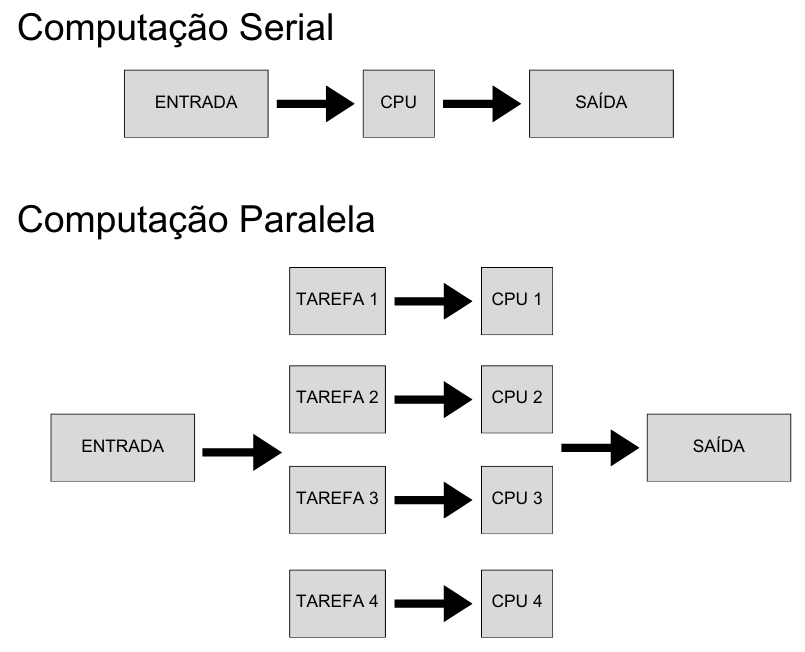
\includegraphics[width=0.5\linewidth]{tcc//img/computacao_serial_paralela.png}
        \caption{Visualização dos conceitos de computação serial e paralela.}
    \label{fig:computacao_serial_paralela}
\end{figure}

Exemplificando com o primeiro caso, foram implementadas duas funções de cálculo de forças: \verb|forcas_seq| e \verb|forcas_par|\footnote{O código completo consta em \cite{potalej_gravidade-fortran}.}. O núcleo do cálculo sequencial é feito da seguinte maneira:

\lstinputlisting[language=Fortran, caption=Código central da função sequencial de forças.]{tcc/codigos/forcas_seq.f90}

O valor \verb|distancia_inv| é o cubo do inverso da distância euclidiana entre os corpos, e \verb|Rab| é o vetor $\vet q_b - \vet q_a$. Observe como os \textit{loops} com \verb|DO| caracterizam a ordem quadrática dos cálculos. A proposta da paralelização neste caso está em dividir o cálculo da força para cada corpo entre os \textit{CPUs}, e posteriormente somar o resultado em um único vetor. Para isso, a biblioteca OpenMP permite definir variáveis compartilhadas (\verb|SHARED|, com as forças totais) e variáveis privadas (\verb|PRIVATE|, variáveis locais), o que garante que nenhuma CPU sobrescreva o vetor de forças das outras CPUs. A função paralelizada é semelhante à sequencial:

\lstinputlisting[language=Fortran, caption=Código central da função paralelizada de forças.]{tcc/codigos/forcas_par.f90}

Na figura \ref{fig:logtempo_paralelo_vs_sequencial} apresentamos um histograma em escala logarítmica com o tempo de computação (em segundos) para diferentes valores de $N$ com o método de Verlet e sem o uso de correção e de colisões, para garantir que o tempo esteja ligado diretamente com o cálculo das forças e do potencial. É possível observar que a diferença é expressiva para valores de $N$ a partir da centena, embora o cenário seja o oposto para valores de $N$ pequenos, uma vez que o custo de distribuir os cálculos entre os núcleos é maior que o do cálculo sequencial.

\begin{figure}
    \centering
    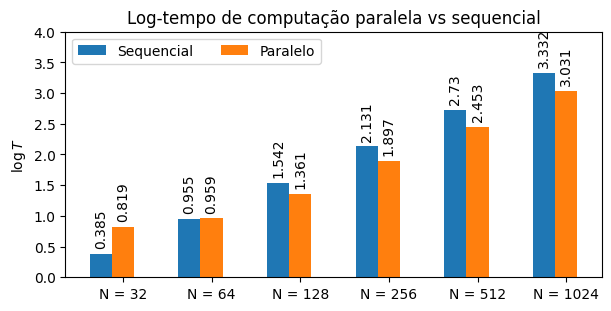
\includegraphics[width=0.8\linewidth]{tcc//img/logtempo.png}
    \caption{Log-tempo de computação paralela e computação sequencial para diferentes valores de $N$ e integração com método de Verlet, sem correção e sem colisão. Foram disponibilizados 4 núcleos para a paralelização.}
    \label{fig:logtempo_paralelo_vs_sequencial}
\end{figure}


%%%%%%%%%%%%%%%%%%%%%%%%%%%%%%%%%%%%%
%%% ARMAZENAMENTO
%%%%%%%%%%%%%%%%%%%%%%%%%%%%%%%%%%%%%
\subsection{Entrada e saída de dados}
Era objetivo que o programa final não contivesse somente simulações, mas facilitasse a geração de valores iniciais e a visualização dos dados também. Nesse sentido, há algumas opções disponíveis para a execução do programa, conforme tabela \ref{tabela:opcoes_entrada}.

\begin{table}
    \centering
    \begin{tabular}{c|c}
        \hline\hline
         \verb|-sv|, \verb|--sorteio-salvar|   & Sorteio de valores iniciais apenas \\
         \verb|-s|, \verb|--sorteio|           & Sorteio de valores iniciais e simulação \\
         \verb|-vi|, \verb|--valores-iniciais| & Simulação a partir de valores iniciais definidos \\
         \verb|-e|, \verb|--exibir|            & Exibição de trajetórias de uma simulação \\
         \verb|-d|, \verb|--dados|             & Exibição de dados de simulação \\
         \hline\hline
    \end{tabular}
    \caption{Opções de entrada no programa final.}
    \label{tabela:opcoes_entrada}
\end{table}

Existem também alguns tipos de arquivos diferentes utilizados pelo programa, os quais vale mencionar, conforme tabela \ref{tabela:arquivos_gerados}. Os arquivos do tipo 1 não são gerados, pois são o tipo mais simples, contendo informações como quantidade de corpos, valor das integrais primeiras, métodos \textit{etc}, sem definir valores iniciais explícitos.

\begin{table}
    \centering
    \begin{tabular}{c|c}
        \hline\hline
         1. & \textit{Preset} para sorteio \\
         2. & \textit{Preset} de valores iniciais \\
         3. & Informações de simulação (\textit{info.txt}) \\
         4. & Dados de simulação (\textit{data.csv}) \\
         \hline\hline
    \end{tabular}
    \caption{Arquivos utilizados ou gerados pelo programa.}
    \label{tabela:arquivos_gerados}
\end{table}

Os arquivos do tipo 1. podem ser usados para gerar valores iniciais explícitos através das chamadas \verb|-sv| e \verb|-s|, que têm entre as saídas um arquivo do tipo 2. Um exemplo de entrada consta no repositório do programa no diretório de \textit{presets}. Existem duas opções para a geração de valores iniciais: o sorteio \textit{comum} e o sorteio de \textit{Hénon}. No primeiro caso, apenas as integrais primeiras são condicionadas conforme o valor desejado. No segundo, são aplicadas as condições de Hénon, conforme descrito na seção \ref{secao:valores_iniciais}.

Já os arquivos de tipo 2 podem ser utilizados para as chamadas \verb|-vi|. Tais arquivos contêm configurações da simulação, como método, tamanho de passo e afins, e também os valores iniciais explícitos. O uso de tais arquivos facilita os testes com diferentes métodos para os mesmos valores iniciais.

Os arquivos de tipo 3 são gerados por simulações em ambas as chamadas \verb|-sv| e \verb|-vi|. Estes contêm informações acerca da simulação em si e de seu desempenho, podendo ser utilizados para comparações entre diferentes métodos. Por não ser um arquivo de entrada, é o que detém mais liberdade para conter diferentes informações. Um exemplo de arquivo de tipo 3 consta no programa \ref{prog:exemplo_saida}.

\lstinputlisting[label={prog:exemplo_saida}, caption={Exemplo de saída do arquivo de informações.}]{tcc/codigos/info.txt}

Por fim, os arquivos de tipo 4 contêm a constante $G$, o tamanho do passo, as massas, e as posições e momentos lineares no decorrer da simulação, armazenados no formato $(x, y, z, p_x, p_y, pz)$. Tais arquivos têm o formato \textit{.csv} (\textit{comma-separated values}). Esta não é a forma mais eficiente de armazenar dados do tipo, uma vez que a escrita de arquivos pelo Fortran é computacionalmente custosa e os arquivos ficam pesados. Para lidar com isso, existem tipos de arquivo mais eficientes, como o HDF\footnote{\textit{Hierarchical Data Format}. Para mais detalhes, veja: \href{https://www.hdfgroup.org/solutions/hdf5/}{https://www.hdfgroup.org/solutions/hdf5/}.}, mas por dificuldades técnicas e a facilidade de manipulação de CSV, a opção mais lenta foi escolhida.

%%%%%%%%%%%%%%%%%%%%%%%%%%%%%%%%%%%%%%%
%%% VALORES INICIAIS
%   Geracao de valores iniciais para o PNC. Condicionamento
%   de integrais primeiras, condições de Hénon, distribuições
%   para massas, posições e momentos.
%%%%%%%%%%%%%%%%%%%%%%%%%%%%%%%%%%%%%%%
%%%%%%%%%%%%%%%%%%%%%%%%%%%%%%%%%%%%%%%
%%% VALORES INICIAIS
%   Geracao de valores iniciais para o PNC. Condicionamento
%   de integrais primeiras, condições de Hénon, distribuições
%   para massas, posições e momentos.
%%%%%%%%%%%%%%%%%%%%%%%%%%%%%%%%%%%%%%%
\section{Valores iniciais}\label{secao:valores_iniciais}

O programa foi elaborado de modo que é possível entrar com valores iniciais de duas maneiras: diretamente e através de sorteios. Da primeira forma, é necessário informar cada massa, posição e momento linear inicial para cada corpo, o que é prático para problemas de poucos corpos mas inviável, a priori, conforme $N$ cresce, sendo necessário utilizar da segunda forma. Vale ressaltar que o sorteio também gera um arquivo de valores iniciais, então a primeira forma pode ser utilizada a posteriori.

Para gerar valores iniciais aleatórios é preciso escolher critérios que atendam as necessidades do problema que se objetiva simular. Para além de gerar valores utilizando, por exemplo, uma distribuição uniforme, muitas vezes é necessário também condicionar os valores gerados de modo que atendam determinada demanda, como os valores das integrais primeiras ou critérios iniciais para um sistema poder ser estável ou não. Tratamos esses dois casos a seguir.

%%%%%%%%%%%%%%%%%%%%%%%%%%%%%%%%%%%%%%%%%%%%%%%%%%%%
\subsection{Condicionamento das integrais primeiras}
Considere valores iniciais $(\vet m, \vet q, \vet p) \in \R_+^N \times \R^{3N} \times \R^{3N}$ obtidos através de um gerador com uma distribuição de probabilidade qualquer, que tenha integrais primeiras $E$, $\vet J$, $\vet P$ e $\vet G$, sendo $\vet G(t) = M \vet q_{cm} (t) - t \vet P$.

Começando por $\vet G$, é importante lembrar que o PNCG tem equações de movimento autônomas, então no instante inicial tem-se $\vet G = M \vet q_{cm}$. Assim, para obter $\tilde{\vet G}$ desejado basta que
\begin{equation*}
    \vet q_{cm}(0) = \dfrac{1}{M} \tilde{\vet G},
\end{equation*}
e para obter tal centro de massas basta transladar as coordenadas $\vet q_a$ individualmente:
\begin{equation*}
    \tilde{\vet q_a} = \vet q_a - \dfrac{1}{M} \left(\vet q_{cm}(0) - \tilde{\vet G}\right).
\end{equation*}

Como já dito anteriormente, o PNCG também é invariante por translações, uma vez que o potencial $V$ o é. Isso significa que utilizar como condição inicial $\vet q$ ou $\tilde{\vet q}$ não afeta a forma como o sistema evoluirá. Assim, uma facilidade bastante conveniente, como já feito anteriormente, é começar com o centro de massas na origem:
\begin{equation}\label{eq:condicionamento_rcm}
    \tilde{\vet q_a} = \vet q_a - \dfrac{1}{M} \vet q_{cm}(0)
    \Rightarrow
    \tilde{\vet G} = \vet 0.
\end{equation}

No caso de $\vet P$, para gerar um $\tilde{\vet P}$ é necessário obter $\tilde{\vet p}$ tal que $\tilde{\vet P} = \sum_{a=1}^{N} \tilde{\vet p_a}$. Então:
\begin{equation*}
    \tilde{\vet P} 
    = \vet P - \vet P + \tilde{\vet P}
    = \sum_{a=1}^{N} \vet p_a - \dfrac{c_a}{C}\left(\vet P - \tilde{\vet P}\right),
    \quad
    C = \sum_{a=1}^{N} c_a,
    \quad
    c_a > 0, \forall a.
\end{equation*}
As constantes $c_a$ podem ser quaisquer, correspondendo a pesos atribuídos a cada momento linear. No caso do PNCG, uma escolha conveniente de pesos é a massa de cada corpo, sendo então
\begin{equation}\label{eq:condicionamento_p}
    \tilde{\vet p_a} = \vet p_a - \dfrac{m_a}{M} (\vet P - \tilde{\vet P}).
\end{equation}

Para o momento angular total $\vet J$, embora para problemas planares baste aplicar 
\begin{equation*}
    \tilde{\vet p_a} = \vet p_a - \dfrac{m_a}{I} \vet q_a \times (\vet J - \tilde{\vet J})
\end{equation*}
para obter $\tilde{\vet J}$, no caso geral em três dimensões a situação é mais complicada. 

\begin{figure}
    \centering
    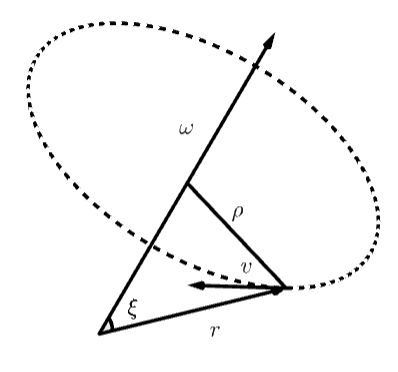
\includegraphics[width=0.3\linewidth]{tcc//img/rotacao.png}
    \caption{Situação descrita.}
    \label{fig:angular_rotacao}
\end{figure}

Considere uma partícula com posição $\vet r$ e um vetor $\vet \omega$ que define um eixo de rotação, do qual $\vet r$ se distancia em $\vet \rho$ e forma um ângulo $\xi$ e cuja velocidade da partícula a relação a é $\vet v$, como na figura \ref{fig:angular_rotacao}. Nessa situação, temos que $\norma{\vet v} = \rho \norma{\vet \omega}$ e $\sin \xi = \rho / \norma{\vet r}$. Uma vez que $\vet v \perp \vet \omega$ e $\vet v \perp \vet r$, podemos concluir que $\vet v \parallel \vet r \times \vet \omega$. Mais ainda, temos que:
\begin{equation*}
    \norma{\vet r \times \vet \omega} 
    = \norma{\vet r} \norma{\vet \omega} \sin \xi
    = \rho \norma{\vet \omega} = \norma{\vet v},
\end{equation*}
então
\begin{equation}\label{eq:velocidade_angular}
    \vet v = \vet r \times \vet \omega.
\end{equation}

O momento angular $\vet J$ também é um vetor perpendicular a $\vet r$ e a $\vet v$, mas $\vet J$ e $\vet \omega$ só são colineares quando $\vet r \perp \vet \omega$. Porém, a partir de (\ref{eq:velocidade_angular}), tem-se que $\vet J = m \vet r \times (\vet r \times \omega)$, então é possível construir um operador $\vet I: \R^3 \to \R^3$ a partir de $m$ e $\vet r$ que leva $\vet \omega$ em $\vet J$ como segue. Veja que
\begin{equation*}
    \vet r \times \vet \omega = (r_2 \omega_3 - r_3 \omega_2) \hat e_1 + (r_3 \omega_1 - r_1 \omega_3) \hat e_2 + (r_1 \omega_2 - r_2 \omega_1) \hat e_3,
\end{equation*}
então
\begin{align*}
    \vet J = m \vet r \times (\vet r \times \vet \omega) &=
    m \begin{bmatrix}
        r_2 r_1 \omega_2 - r_2^2 \omega_1 - r_3^2 \omega_1 + r_1 r_3 \omega_3 \\
        r_3 r_2 \omega_3 - r_3^2 \omega_2 - r_1^2 \omega_2 + r_1 r_2 \omega_1 \\
        r_1 r_3 \omega_1 - r_1^2 \omega_3 - r_2^2 \omega_3 + r_2 r_3 \omega_2
    \end{bmatrix} \\ &=
    m \begin{bmatrix}
        -(r_2^2 + r_3^2) & r_1 r_2 & r_1 r_3 \\
        r_1 r_2 & -(r_1^2 + r_3^2) & r_2 r_3 \\
        r_1 r_3 & r_2 r_3 & - (r_1^2 + r_2^2)
    \end{bmatrix}
    \begin{bmatrix}
        \omega_1 \\ \omega_2 \\ \omega_3
    \end{bmatrix}
    := \vet I \vet \omega.
\end{align*}

Tal aplicação $\vet I$ já é bem conhecida na literatura pelo nome de \textit{tensor de inércia}, fornecendo uma nova expressão para o momento angular. No caso de diversos corpos, a ideia é definir um eixo de rotação comum e a partir dele aplicar transformações sobre a velocidade angular de cada corpo. A primeira parte é simples, pois
\begin{equation*}
    \vet J = \sum_{a=1}^{N} \vet J_a = \sum_{a=1}^{N} \vet I_a \vet \omega = \vet I_{total} \vet \omega.
\end{equation*}

A partir disso, para obter um momento angular desejado $\tilde{\vet J}$ basta encontrar um eixo $\vet \omega$ tal que
\begin{equation*}
    \vet I_{total} \vet \omega = \vet J - \tilde{\vet J}
\end{equation*}
e aplicar a transformação
\begin{equation}\label{eq:condicionamento_j}
    \tilde{\vet p_a} = \vet p_a - m_a \vet q_a \times \vet \omega.
\end{equation}

A essa altura, é natural suspeitar que aplicar (\ref{eq:condicionamento_j}) depois de (\ref{eq:condicionamento_p}) mudaria o valor de $\tilde{\vet P}$ e vice-versa. Porém, considere o misto das aplicações:
\begin{equation}\label{eq:condicionamento_j_p}
    \tilde{\vet p_a} = \vet p_a - \dfrac{m_a}{M}(\vet P - \tilde{\vet P}) - m_a \vet q_a \times \omega.
\end{equation}

Temos:
\begin{align*}
    \sum_{a=1}^{N} \tilde{\vet p_a}
    & = \tilde{\vet P} - \vet q_{cm} \times \omega = \tilde{\vet P}
    \\
    \sum_{a=1}^{N} \vet q_a \times \tilde{\vet p_a}
    & = \tilde{\vet J} - \dfrac{1}{M} \vet q_{cm} \times (\vet P - \tilde{\vet P}) = \tilde{\vet J},
\end{align*}
pois $\vet q_{cm} = \vet 0$. Assim, com o centro de massas na origem, é possível condicionar o momento linear total e o momento angular total separadamente.

Já para a energia total $E$, existem dois caminhos possíveis: aplicar transformações sobre as posições ou sobre os momentos lineares. Uma vez que $E$ é separável, isto é,
\begin{equation*}
    E(\vet q, \vet p) = T(\vet p) + V(\vet q),
\end{equation*}
e que as funções $T$ e $V$ têm sinais opostos no PNCG, existem muitas formas diferentes de balancear a energia total. Para obter uma energia total negativa, por exemplo, basta aproximar os corpos, mas pode ser suficiente reduzir as velocidades em vez disso. Já para uma energia total positiva, basta aumentar as velocidades, mas também pode ser possível apenas distanciar os corpos. No geral, tomando $\tilde{\vet q} = \alpha^{-1} \vet q$ e $\tilde{\vet p} = \beta \vet p$, tem-se:
\begin{equation*}
    \tilde E := E(\tilde{\vet q}, \tilde{\vet p}) = \beta^2 T(\vet p) + \alpha V (\vet q) = \beta^2 (E_0 - V_0) + \alpha V_0.
\end{equation*}

Neste trabalho, a solução aplicada para esse dilema foi aplicar a transformação necessária para as velocidades, e se a energia desejada for diferente de zero então é aplicada uma aproximação ou distanciamento entre os corpos. Na prática, isso foi dado pelo seguinte:
\begin{equation*}
    \beta = \sqrt{\dfrac{-V_0}{T(\vet p_0)}},
    \quad
    \alpha = 1 + \dfrac{\tilde E}{V_0}
\end{equation*}
Um questionamento cabível é o quanto essa escolha afetou os resultados obtidos, uma vez que existem diversas outras transformações possíveis. Não chegamos a testar outros valores, então no momento não temos resposta para isso. 

A transformação que condiciona a energia total afeta os momentos linear e angular totais:
\begin{equation*}
    \sum_{a=1}^{N} \tilde{\vet p_a} = \beta \vet P,
    \quad
    \sum_{a=1}^{N} \tilde{\vet q_a} \times \tilde{\vet p_a} = \dfrac{\beta}{\alpha} \vet J.
\end{equation*}

Este problema é de fácil resolução, pois basta que $\tilde{\vet P}$ e $\tilde{\vet J}$ sejam multiplicados pelas devidas constantes na equação (\ref{eq:condicionamento_j_p}), gerando a seguinte mudança de coordenadas:
\begin{align}
    \tilde{\vet q_a} &= \dfrac{1}{\alpha}\left(\vet q_a - \dfrac{1}{M} \vet q_{cm} (0)\right), \\
    \tilde{\vet p_a} &= \beta\left( \vet p_a - \dfrac{m_a}{M} \left(\vet P - \dfrac{\tilde P}{\beta}\right) - m_a \vet q_a \times \vet \omega \right), \\
    \vet I_{total} \vet \omega &= \vet J - \dfrac{\tilde{\vet J} \alpha}{\beta}, \\
    \alpha = 1 + \dfrac{\tilde E}{V_0}, 
    & \quad
    \label{eq:beta_1} \beta = \sqrt{\dfrac{- V_0}{T( \tilde{\vet p_a} / \beta)}}
\end{align}

Observe que $\beta$ fica definido implicitamente pela equação (\ref{eq:beta_1}). Elevando os dois lados ao quadrado é possível isolar $\beta$, obtendo-se a seguinte expressão:
\begin{equation}
    \beta = \pm \sqrt{- \dfrac{V_0 + S_2}{S_1}},
\end{equation}
onde
\begin{align*}
    S_1 &= \sum_{a=1}^{N} \dfrac{1}{2 m_a} \norma{\vet K_1^a}^2 
    = \sum_{a=1}^{N} \dfrac{1}{2 m_a} \norma{\vet p_a - \dfrac{m_a}{M} \vet P - m_a q_a \times (\bm I_{total}^{-1} \vet J)}^2, 
    \\
    S_2 &= \sum_{a=1}^{N} \dfrac{1}{2 m_a} \norma{\vet K_2^a}^2
    = \sum_{a=1}^{N} \dfrac{1}{2 m_a} \norma{\dfrac{m_a}{M} \tilde{\vet P} + \alpha m_a \vet q_a \times (\bm I_{total}^{-1} \tilde{\vet J})}^2,
    \\
    \sum_{a=1}^{N} & \dfrac{1}{m_a} \prodint{\vet K_1^a}{\vet K_2^a} = 0.
\end{align*}

A escolha do sinal de $\beta$ define a evolução do sistema, uma vez que a velocidade de cada partícula é multiplicada por $\beta$. O sistema com $\beta < 0$ é o equivalente de simular o caso $\beta > 0$ utilizando um tamanho de passo $h^- < 0$ para integradores reversíveis, ou seja, escolhido um sinal de $\beta$, o seu oposto equivale a integrar o sistema no sentido temporal oposto. Em termos de posições, porém, conseguimos uma única configuração que atende às expectativas de integrais primeiras e tem centro de massas centrado na origem. Veja um exemplo do mencionado na figura \ref{fig:vi-betas}.

\begin{figure}
    \centering
    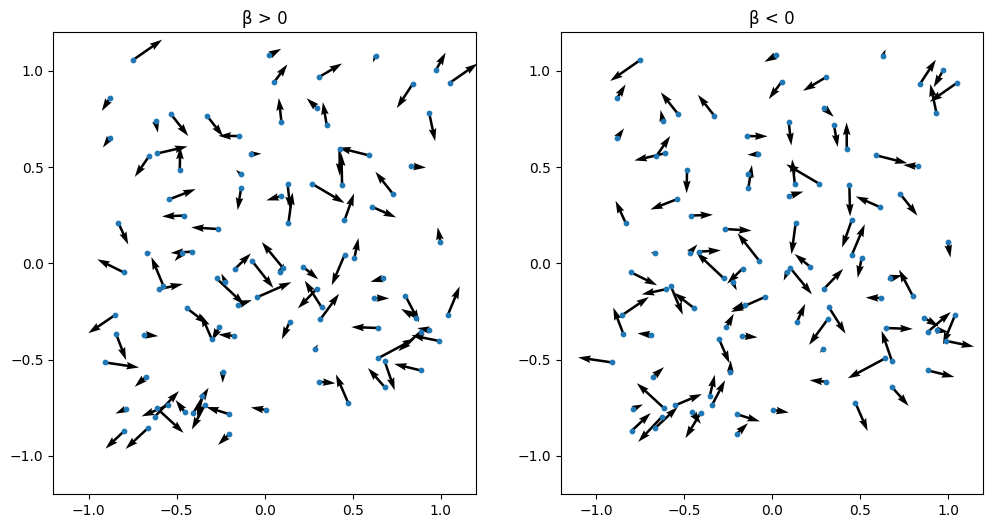
\includegraphics[width=0.8\linewidth]{tcc//img/100corpos_betas.png}
    \caption{Posições e momentos lineares em um problema de 100 corpos com todas as integrais primeiras nulas para os dois valores de $\beta$.}
    \label{fig:vi-betas}
\end{figure}




%%%%%%%%%%%%%%%%%%%%%%%%%%%%%%%%%%%%%%
\subsection{Condições de estabilidade}\label{subsection:condicoes_aarseth}
Em busca de um sistema de unidades padrão que permitisse a comparação de resultados obtidos por diferentes pesquisadores do PNCG, \citep{Hnon1972, Heggie} propõem utilizar o seguinte:
\begin{equation*}
    G = 1, \quad
    M = 1, \quad
    R_V = 1.
\end{equation*}
sendo $R_V$ o raio de virial. Isso significa que temos o seguinte, conforme equação (\ref{eq:raio_virial}):
\begin{equation*}
    V \approx - \dfrac{G M^2}{2 R_V} = - \dfrac{1}{2},
\end{equation*}
e pelo Teorema do Virial (Teorema \ref{teorema:virial}) para uma relação de equilíbrio instantânea:
\begin{equation*}
    T = - \dfrac{1}{2} V \approx \dfrac{1}{4} 
    \Rightarrow
    E = - \dfrac{1}{4}.
\end{equation*}

Para sistemas com essas condições iniciais, é esperado que, com alguma regularização em uso (como o amortecimento do potencial, por exemplo), o sistema fique limitado - ou seja, \textit{estável} -, ao menos temporariamente.

Os testes apresentados nas próximas subseções nos quais as massas são iguais e somam 1 utilizam as condições de Hénon.


%%%%%%%%%%%%%%%%%%%%%%%%%%%%%%%%%%%%%%%
%%% COLISOES
%   Aplicacao das colisoes e criterios. Exemplos do uso
%   para problemas de poucos corpos e problemas de varios
%   corpos. Custo computacional e eficiencia.
%%%%%%%%%%%%%%%%%%%%%%%%%%%%%%%%%%%%%%%
%%%%%%%%%%%%%%%%%%%%%%%%%%%%%%%%%%%%%%%
%%% COLISOES
%   Aplicacao das colisoes e criterios. Exemplos do uso
%   para problemas de poucos corpos e problemas de varios
%   corpos. Custo computacional e eficiencia.
%%%%%%%%%%%%%%%%%%%%%%%%%%%%%%%%%%%%%%%
\section{Colisões}\label{section:simulacao_colisoes}
Como inicialmente discutido na seção \ref{section:pncg_colisoes}, existem algumas formas de lidar com colisões no PNCG e que se aplicam para aproximações muito intensas, ou \textit{quase colisões}, uma vez que o conjunto de valores iniciais que levam a uma colisão em tempo finito têm medida zero. A abordagem com colisões elásticas é uma delas.

Para utilizar colisões, como já dito, um meio natural é definir uma densidade $\rho$ para a massa de modo que
\begin{equation}
    r_a = \sqrt[3]{\dfrac{3 m_a}{4 \pi \rho}}
\end{equation}
é o raio de um corpo esférico de massa $m_a$. Cada escolha de densidade possível gera um conjunto de trajetórias diferentes, uma vez que uma aproximação intensa que é considerada como colisão para um certo $\rho_1$ pode não o ser para um $\rho_2$ diferente. Porém, este método possui a vantagem de garantir a reprodutibilidade das simulações.

Um problema de utilizar colisões elásticas é que nem sempre o raio é o suficiente para detectar uma colisão ou quase-colisão antes que o estrago numérico seja feito. Pode acontecer, por exemplo, de em um instante $t$ dois corpos estarem distantes o suficiente para não haver colisão mas no instante $t + \delta t$ os dois volumes associados aos corpos terem uma interseção não vazia no espaço de configurações - na prática, um corpo \textit{entrar} no outro, como na figura \ref{fig:colisao_intersecao}. Uma tática que pode ser utilizada para evitar isso é: uma vez detectada a interseção, interpolar as trajetórias entre os instantes $t$ e $t+\delta t$, obtendo assim o exato momento da colisão $t \leq t^* \leq t+\delta t$, aplicar a colisão em $t^*$ e substituir a trajetória com interseção em $t + \delta t$ pela trajetória em que houve colisão no instante $t^*$. Embora não exista dificuldade teórica em tal tática, aplicá-la numericamente é um desafio, especialmente em problemas de muitos corpos, pois todo esse processo é, além de custoso, computacionalmente complicado de ser avaliado, por isso não foi utilizado.

\begin{figure}
    \centering
    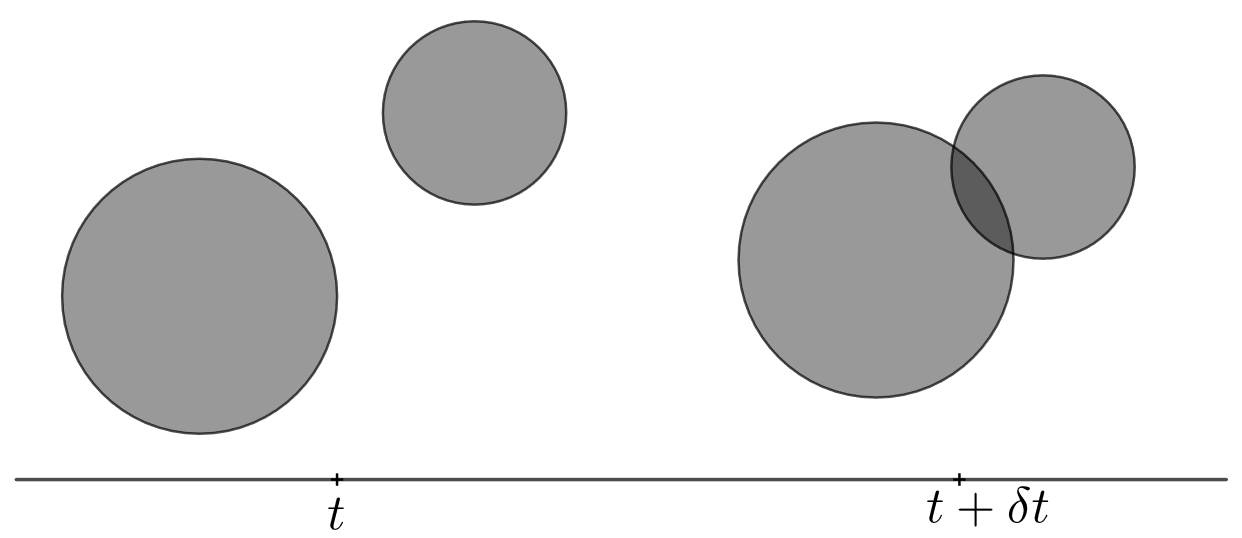
\includegraphics[width=0.7\linewidth]{tcc//img/colisao_intersecao.png}
    \caption{Problema descrito, onde o instante de colisão exato $t^*$ é tal que $t \leq t^* \leq t + \delta t$}
    \label{fig:colisao_intersecao}
\end{figure}

Outra saída mais simples para o problema é: uma vez detectada uma aproximação no instante $t+\delta t$ intensa o suficiente para desestabilizar numericamente o sistema antes de uma colisão elástica surtir efeito, voltar para o instante $t$ e aplicar a colisão elástica neste instante. Existem dois problemas com essa tática: é preciso escolher mais um valor $\epsilon_E$ (ligado à energia) para poder definir o que é uma \textit{desestabilização} considerável e é possível que retornar ao passo anterior resolva o problema de imediato, mas jogue a partícula colidida em rota de colisão com outra partícula, gerando uma situação recursiva.

O primeiro problema poderia ser resolvido com estatística, identificando uma ``desestabilização'' como um \textit{outlier} numa estatística suficiente para a energia, por exemplo, ou com o rigor dos integradores numéricos, pois cada integrador tem um teto para o erro das trajetórias e consequentemente um teto para o erro da energia total, sendo uma ``desestabilização'' qualquer coisa acima dessa margem. A solução estatística chegou a ser brevemente testada mas não ofereceu resultados satisfatórios, uma vez que trouxe mais um custo computacional e não foi capaz de se livrar do segundo problema. A solução com teto dos integradores não foi implementada por dificuldades teóricas em determinar o teto, mas pretendemos avaliar essa medida de erro de cada método no futuro.

Uma última questão com as colisões elásticas é o custo de identificar seu acontecimento. Da mesma forma que o potencial e as forças, são necessárias $N (N-1) / 2$ verificações para identificar uma colisão, sendo então mais uma operação computacionalmente custosa. Existem outras formas mais eficientes de detectar colisões e há toda uma literatura voltada para isso, como \cite{Ericson2005}, pois existe uma gama de aplicações que necessitam de métodos eficientes para detecção de colisões. Para este trabalho, por facilidade, foi utilizada a verificação um-a-um comentada.

Existem outras regularizações que permitem lidar com colisões, especialmente colisões binárias, como a transformação de Levi-Civita (para problemas planares), sua generalização no método de Kustaanheimo-Stiefel e a alternativa pelo método de Burdet-Heggie \citep{aarseth_gravitational_2003}. Nenhuma dessas regularizações foi estudada a fundo então estas não serão tratadas neste trabalho. Para mais detalhes, a referência de Aarseth é recomendada para os três métodos mencionados, tendo o seu capítulo 4 totalmente voltado para este problema.

Há também outra forma de evitar colisões e quase-colisões, que é impondo um limite sobre o potencial. Tomando $\epsilon > 0$, definimos o potencial amortecido
\begin{equation}
    V_\epsilon = - G \sum_{a < b} \dfrac{m_a m_b}{\sqrt{r_{ab}^2 + \epsilon^2}},
\end{equation}
o que gera as forças
\begin{equation}
    \derpar{V}{\vet q_a} = G \sum_{b \neq a} m_a m_b \dfrac{\vet q_b - \vet q_a}{(r_{ab}^2 + \epsilon^2)^{3/2}}.
\end{equation}

Observe que apesar da diferença nos cálculos, a energia total amortecida $E_\epsilon = T + V_\epsilon$ ainda é conservada, pois
\begin{equation*}
    \der{E_\epsilon}{t} 
    = \nabla_{\vet p} T \cdot \dvet p + \nabla_{\vet q} V_\epsilon \cdot \dvet q
    = 0.
\end{equation*}

O uso de um amortecimento pode levantar dúvidas naturais a respeito da precisão dos resultados obtidos com simulações. É fato que o mesmo conjunto de valores iniciais leva a um resultado quando usado o potencial $V$ e a outro resultado quando usado o potencial $V_\epsilon$. Porém, quando o interesse está nas propriedades dinâmicas do sistema e não em trajetórias individuais - o que no geral ocorre para valores de $N$ suficientemente grandes -, $\epsilon$ precisa ser relativamente grande para que o resultado final seja notavelmente diferente \citep[235]{aarseth_gravitational_2003}.

Dessa forma, tanto a colisão elástica quanto o potencial amortecido conservam a energia de alguma forma, então foram implementados no programa final. Cabe observar que uma possível solução para se livrar de alguns dos problemas comentados no uso de colisões elásticas é utilizar um método híbrido que incorpore o amortecimento, além de utilizar o corretor para amenizar a instabilidade do potencial. Ainda assim, é esperado que as órbitas individuais sejam diferentes, mesmo que as integrais primeiras sejam as mesmas. Um exemplo pode ser visto na figura \ref{fig:iau25_trajetorias_colisoes}.

\begin{figure}
    \centering
    \begin{subfigure}{.5\textwidth}
      \centering
      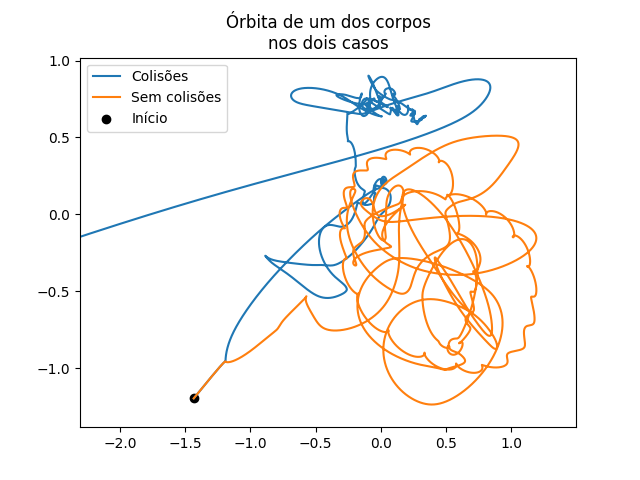
\includegraphics[width=\linewidth]{tcc/img/trajetoria_iau25_colisao_vs_sem_colisao.png}
      % \caption{Órbita de um dos corpos nos dois casos.}
      \caption{}
      \label{fig:iau25_trajetorias_colisoes_a}
    \end{subfigure}%
    \begin{subfigure}{.5\textwidth}
      \centering
      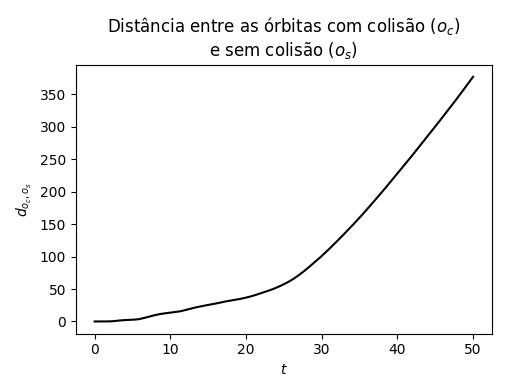
\includegraphics[width=\linewidth]{tcc/img/distancia_orbitas_iau25.png}
      % \caption{Distância entre as órbitas no espaço de fases.}
      \caption{}
      \label{fig:iau25_trajetorias_colisoes_b}
    \end{subfigure}
    
    \caption{Simulações do problema-modelo \ref{probmodelo:iau25} via método RKN671 com $h=10^{-3}$, $\epsilon=5h$ e corretor com margem de erro da energia $10^{-10}$ no intervalo $[0,50]$. Em um dos casos utilizou-se colisões ativadas com $r_a = 5h$, $a=1,2,...,N$ e no outro as colisões estavam desativadas.}
    \label{fig:iau25_trajetorias_colisoes}
\end{figure}

%%%%%%%%%%%%%%%%%%%%%%%%%%%%%%%%%%%%%%%
%%% SOBRE O CORRETOR NUMÉRICO
%   Questões práticas do corretor
%%%%%%%%%%%%%%%%%%%%%%%%%%%%%%%%%%%%%%%
%%%%%%%%%%%%%%%%%%%%%%%%%%%%%%%%%%%%%%%
%%% Corretor numérico
%   Questões práticas sobre o uso do
%   corretor numérico.
%%%%%%%%%%%%%%%%%%%%%%%%%%%%%%%%%%%%%%%
\section{Uso do corretor numérico}\label{secao:uso_do_corretor}
O corretor numérico apresentado na seção \ref{secao:corretor_numerico} possui algumas questões sobre sua usabilidade no programa que valem ser discutidas nesta seção. Para começar, é interessante que o uso de um corretor numérico não eleve drasticamente o tempo necessário para realizar uma simulação. No caso deste corretor, existem alguns custos associados.

O primeiro é no cálculo das integrais primeiras. Embora $\vet \Psi(\vet z_0)$ seja calculado apenas uma vez, a cada iteração que utiliza o corretor é necessário calcular $\vet \Psi(\vet z)$. O cálculo direto da energia total para um potencial de N-corpos, por exemplo, tem ordem $O(N^2)$ de operações, podendo ser então um custo relevante.

Um segundo custo é na resolução do sistema linear (\ref{eq:corretor_equacao_2}), pois a matriz jacobiana $D \vet \Psi$ tem tamanho $k \times 6N$. Observe, porém, que a matriz
\begin{equation}\label{eq:corretor_matriz_normal}
    \vet \Gamma (\vet z) = D \vet \Psi(\vet z) D \vet \Psi(\vet z)^T
\end{equation}
é uma matriz normal, e seu tamanho é $k \times k$. Além disso, cada elemento seu é dado diretamente por um produto interno:
\begin{equation*}
    \vet \Gamma_{ij} = \prodint{\nabla \psi_i}{\nabla \psi_j},
\end{equation*}
o que a caracteriza como uma matriz de Gram, e também em casos com poucas integrais primeiras de interesse isso significa que esta pode ser calculada manualmente, otimizando uma parte do processo. 

Além disso, a resolução do sistema de equações
\begin{equation*}
    \bm \Gamma (\vet y) \vet \alpha = \vet \Psi(\vet z) - \vet \Psi(\vet z_0).
\end{equation*}
também possui um custo associado, o que depende da quantidade de integrais primeiras utilizadas e do método utilizado para resolução. A primeira abordagem computacional tomada foi utilizar a sub-rotina \verb|dgesv|, do LAPACK, a qual resolve um sistema $\bm A \vet x = \vet b$, com $\bm A$ $n \times n$ aplicando a decomposição LU sobre $\bm A$, o que tem custo $O(n^3)$, e resolvendo o sistema triangular restante, com custo $O(n^2)$.

Porém, uma vez que a matriz $\bm \Gamma$ é de Gram, é também no mínimo positiva semi-definida. Isso significa que em vez de utilizar LU, que tem como fundo o pivoteamento gaussiano, faz sentido utilizar a decomposição de Cholesky, que apesar de ter $O(n^3)$ consome apenas metade das operações do pivoteamento gaussiano, e trata-se de um algoritmo que sempre é numericamente estável \citep[172-177]{Trefethen1997}. No LAPACK, as subrotinas utilizadas para isso foram \verb|dpotrf| (para a fatoração de Cholesky) e \verb|dpotrs| (para a resolução de um sistema linear Cholesky-fatorado). 

Realizamos alguns testes com os dois métodos de resolução mas não encontramos diferenças expressivas. Um exemplo de aplicação foi em um problema de $10^3$ corpos com condições de Hénon (ver seção \ref{secao:valores_iniciais}), e o resultado pode ser encontrado na figura \ref{fig:corretor_cholesky_vs_lu_energia} e na tabela \ref{tab:corretor_cholesky_vs_lu_energia}. Vale ressaltar que, quanto ao desempenho, ambas as simulações levaram por volta de 10,4 minutos, com uma pequena vantagem de alguns segundos para o uso de Cholesky.

\begin{figure}
    \centering
    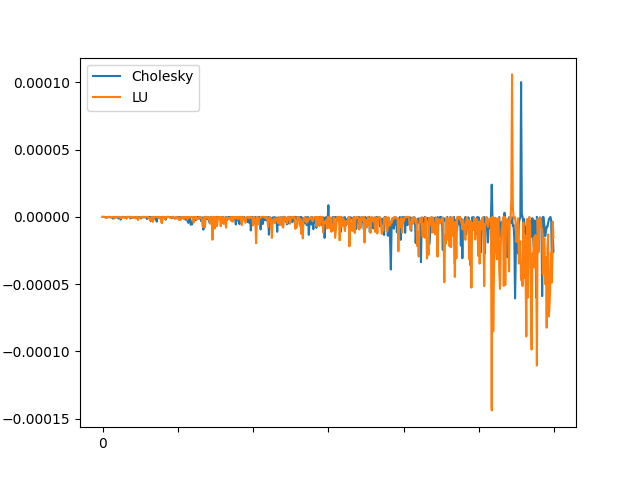
\includegraphics[width=0.5\linewidth]{tcc//img/exemplo_cholesky_vs_lu_energia.png}
    \caption{Variação da energia $\Delta E$ em um problema de $10^3$ corpos utilizando o integrador Velocity-Verlet (2ª ordem), $h=0.1$ e $\epsilon=0.04$, com margem de erro da energia $10^{-11}$.}
    \label{fig:corretor_cholesky_vs_lu_energia}
\end{figure}

\begin{table}[]
    \centering
    \begin{tabular}{c|cc}
                      & Cholesky     & LU           \\ \hline
        Média         & $-3.639 \cdot 10^{-06}$ & $-6.656 \cdot 10^{-06}$ \\
        Mediana       & $-1.208 \cdot 10^{-06}$ & $-1.277 \cdot 10^{-06}$ \\
        Desvio padrão & $8.599 \cdot 10^{-06}$  & $1.551 \cdot 10^{-05}$  
    \end{tabular}
    \caption{Estatísticas sobre o valor $\Delta E$, nas condições da figura \ref{fig:corretor_cholesky_vs_lu_energia}.}
    \label{tab:corretor_cholesky_vs_lu_energia}
\end{table}

Diante do custo, vale questionar também se de fato faz sentido utilizar todas as integrais primeiras no corretor. Por mais que mais informações devam levar a uma correção melhor, uma integral primeira que seja numericamente estável pode ser só um custo a mais e não trazer resultados tão diferentes do que sem o seu uso. 

No PNCG, o centro de massas e o momento linear total são numericamente bem-comportados por serem lineares, e o momento angular também é estável por ser uma expressão livre de singularidades, como exemplificado na figura \ref{fig:var_integrais_es_iau25} da seção \ref{secao:integradores_simpleticos}. A energia total, por outro lado, é bastante instável em aproximações intensas devido ao potencial ser inversamente proporcional às distâncias. Dessa forma, como sugere \cite{Nacozy1972}, aplicar a correção somente na energia total no PNCG é, no geral, suficiente. O vetor de correção $\alpha$ (que é um escalar nesse caso) possui uma forma explícita:
\begin{equation}
    \alpha = \dfrac{E(\vet z) - E(\vet z_0)}{\norma{\nabla E(\vet z)}^2}.
\end{equation}
Um exemplo de aplicação no problema-modelo \ref{probmodelo:iau25} com as duas formas de correção pode ser visualizado na figura \ref{fig:var_energia_iau25_corretores}.

\begin{figure}
    \centering
    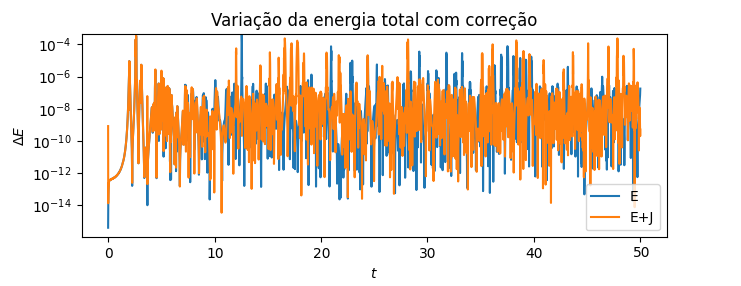
\includegraphics[width=\linewidth]{tcc/img/var_energia_todas_vs_energia_iau25.png}
    % \caption{RKN671 H=0.001, E=0.1, [0,50], COR=1E-10}
    \caption{Variação da energia no problema-modelo \ref{probmodelo:iau25} simulado via método RKN671 com $h=10^{-3}$, $\epsilon = 10^{-1}$ e com margem de erro da energia $10^{-10}$ no intervalo $[0,50]$. Em azul, foi aplicada a correção somente na energia total, enquanto em laranja foi aplicada a correção também no momento angular total.}
    \label{fig:var_energia_iau25_corretores}
\end{figure}

De toda forma, o custo do corretor só ocorre quando este é aplicado, então um bom critério de aplicabilidade pode reduzir o custo do corretor através da sua utilização somente quando estritamente necessário. No problema-modelo utilizado por Nacozy, o corretor era aplicado quando o erro da energia total atingia um valor por volta de 100 vezes menor que o erro de truncamento desejado. Constatamos empiricamente que com o uso do amortecimento no potencial, uma vez que o potencial deixa de ter singularidades, o teto pode ser tanto quanto desejado, então a escolha de Nacozy é razoável para o PNCG.

A implementação do corretor numérico é a sub-rotina \verb|correcao|, que depende de outras sub-rotinas de mecânica do programa.

%%%%%%%%%%%%%%%%%%%%%%%%%%%%%%%%%%%%%%%
%%% OUTROS ASPECTOS PRATICOS DO PNCG [NAO INCLUIDO]
%   Falar do tamanho de passo
%%%%%%%%%%%%%%%%%%%%%%%%%%%%%%%%%%%%%%%
% \section{Outros aspectos práticos do PNCG}

Além do tratado, existem questões práticas da simulação do PNCG que valem ser mencionadas, como a escolha do tamanho de passo. [ Escrever melhor]

A escolha de um tamanho de passo define

%%%%%%%%%%%%%%%%%%%%%%%%%%%%%%%%%%%%%%%
%%% SIMULACAO DA DINAMICA DE FORMAS
%   Falar sobre a simulacao da dinamica
%   de formas
%%%%%%%%%%%%%%%%%%%%%%%%%%%%%%%%%%%%%%%
\section{Aplicação: Dinâmica de Formas}\label{secao:simulacao_dinamica_de_formas}

Na seção \ref{secao:dinamica_de_formas} apresentamos uma breve introdução à Dinâmica de Formas sobre o PNCG, onde introduzimos a \textit{complexidade} $C_S$ como uma medida de evolução de um sistema e também as \textit{coordenadas objetivas} $(\vet \sigma, \vet \pi)$ sobre o espaço de formas. Nesta seção, visualizaremos alguns dos resultados apresentados.

Todas as simulações utilizadas aqui foram feitas com momento angular total $\vet J = \vet 0$, momento linear total $\vet P = \vet 0$ e centro de massas $\vet q_{cm} = \vet 0$. A energia foi testada com diferentes valores para diferentes objetivos, e os valores são explicitados em cada caso.



%%%%%%%% PROBLEMAS DE 3 CORPOS
\subsection{Problemas de 3 corpos}

Para visualizar as coordenadas objetivas $(\vet \sigma, \vet \pi)$, tomamos primeiramente um problema de 3 corpos com uma trajetória simples: um par kepleriano e um corpo ejetado, como na figura \ref{fig:probmodel_3_corpos_energia0_trajetoria}. Trata-se do problema-modelo \ref{probmodelo:3corpos_energia_nula}, integrado no intervalo $[0,50]$ via método de Verlet com $h=10^{-3}$, sem correção.

Este é um sistema com energia total 0, então os resultados da Dinâmica de Formas se aplicam. Por exemplo, a ejeção de um dos corpos corresponde a um atrito no espaço de fases (tomando a coordenada $\vet \omega$). Além disso, a complexidade (figura \ref{fig:3corpos_energia0_complexidade}) aumenta no sentido futuro devido à separação do sistema em dois, embora possua fortes oscilações ligadas às aproximações do sistema binário.

\begin{figure}[H]
    \centering
    
    \begin{subfigure}{.5\textwidth}
        \centering
        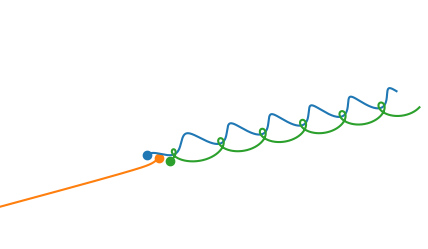
\includegraphics[width=0.8\linewidth]{tcc/img/sd/3corpos_energia0_posicoes_nd_2.png}
        \caption{}
        \label{fig:probmodel_3_corpos_energia0_trajetoria}
    \end{subfigure}%
    \begin{subfigure}{.5\textwidth}
        \centering
        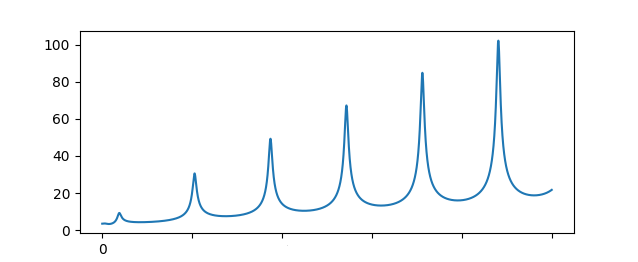
\includegraphics[width=\linewidth]{tcc/img/sd/3corpos_energia0_complexidade.png}
        \caption{}
        \label{fig:3corpos_energia0_complexidade}
    \end{subfigure}

    \caption{Problema-modelo \ref{probmodelo:3corpos_energia_nula}. À esquerda, recorte das trajetórias. À direita, a complexidade apresentada pelo sistema.}
    \label{fig:figuras_probmodel_3_energia0}
\end{figure}

Na figura \ref{fig:3corpos_energia0_posicoes_sd} é possível observar os comportamentos de ejeção e de formação de binários. Embora o corpo ejetado se afaste a princípio, conforme o par binário se forma, o ejetado desacelera e inicia uma trajetória cíclica e dissipativa. E, de fato, conforme a figura \ref{fig:3corpos_energia0_velocidades_sd} mostra, o corpo ejetado está desacelerando, enquanto o momento de forma ($\vet \pi$) dos outros dois apresenta trajetórias circulares com um raio cada vez maior e cada vez mais rapidamente. 

\begin{figure}[H]
    \centering
    \begin{subfigure}{.5\textwidth}
        \centering
        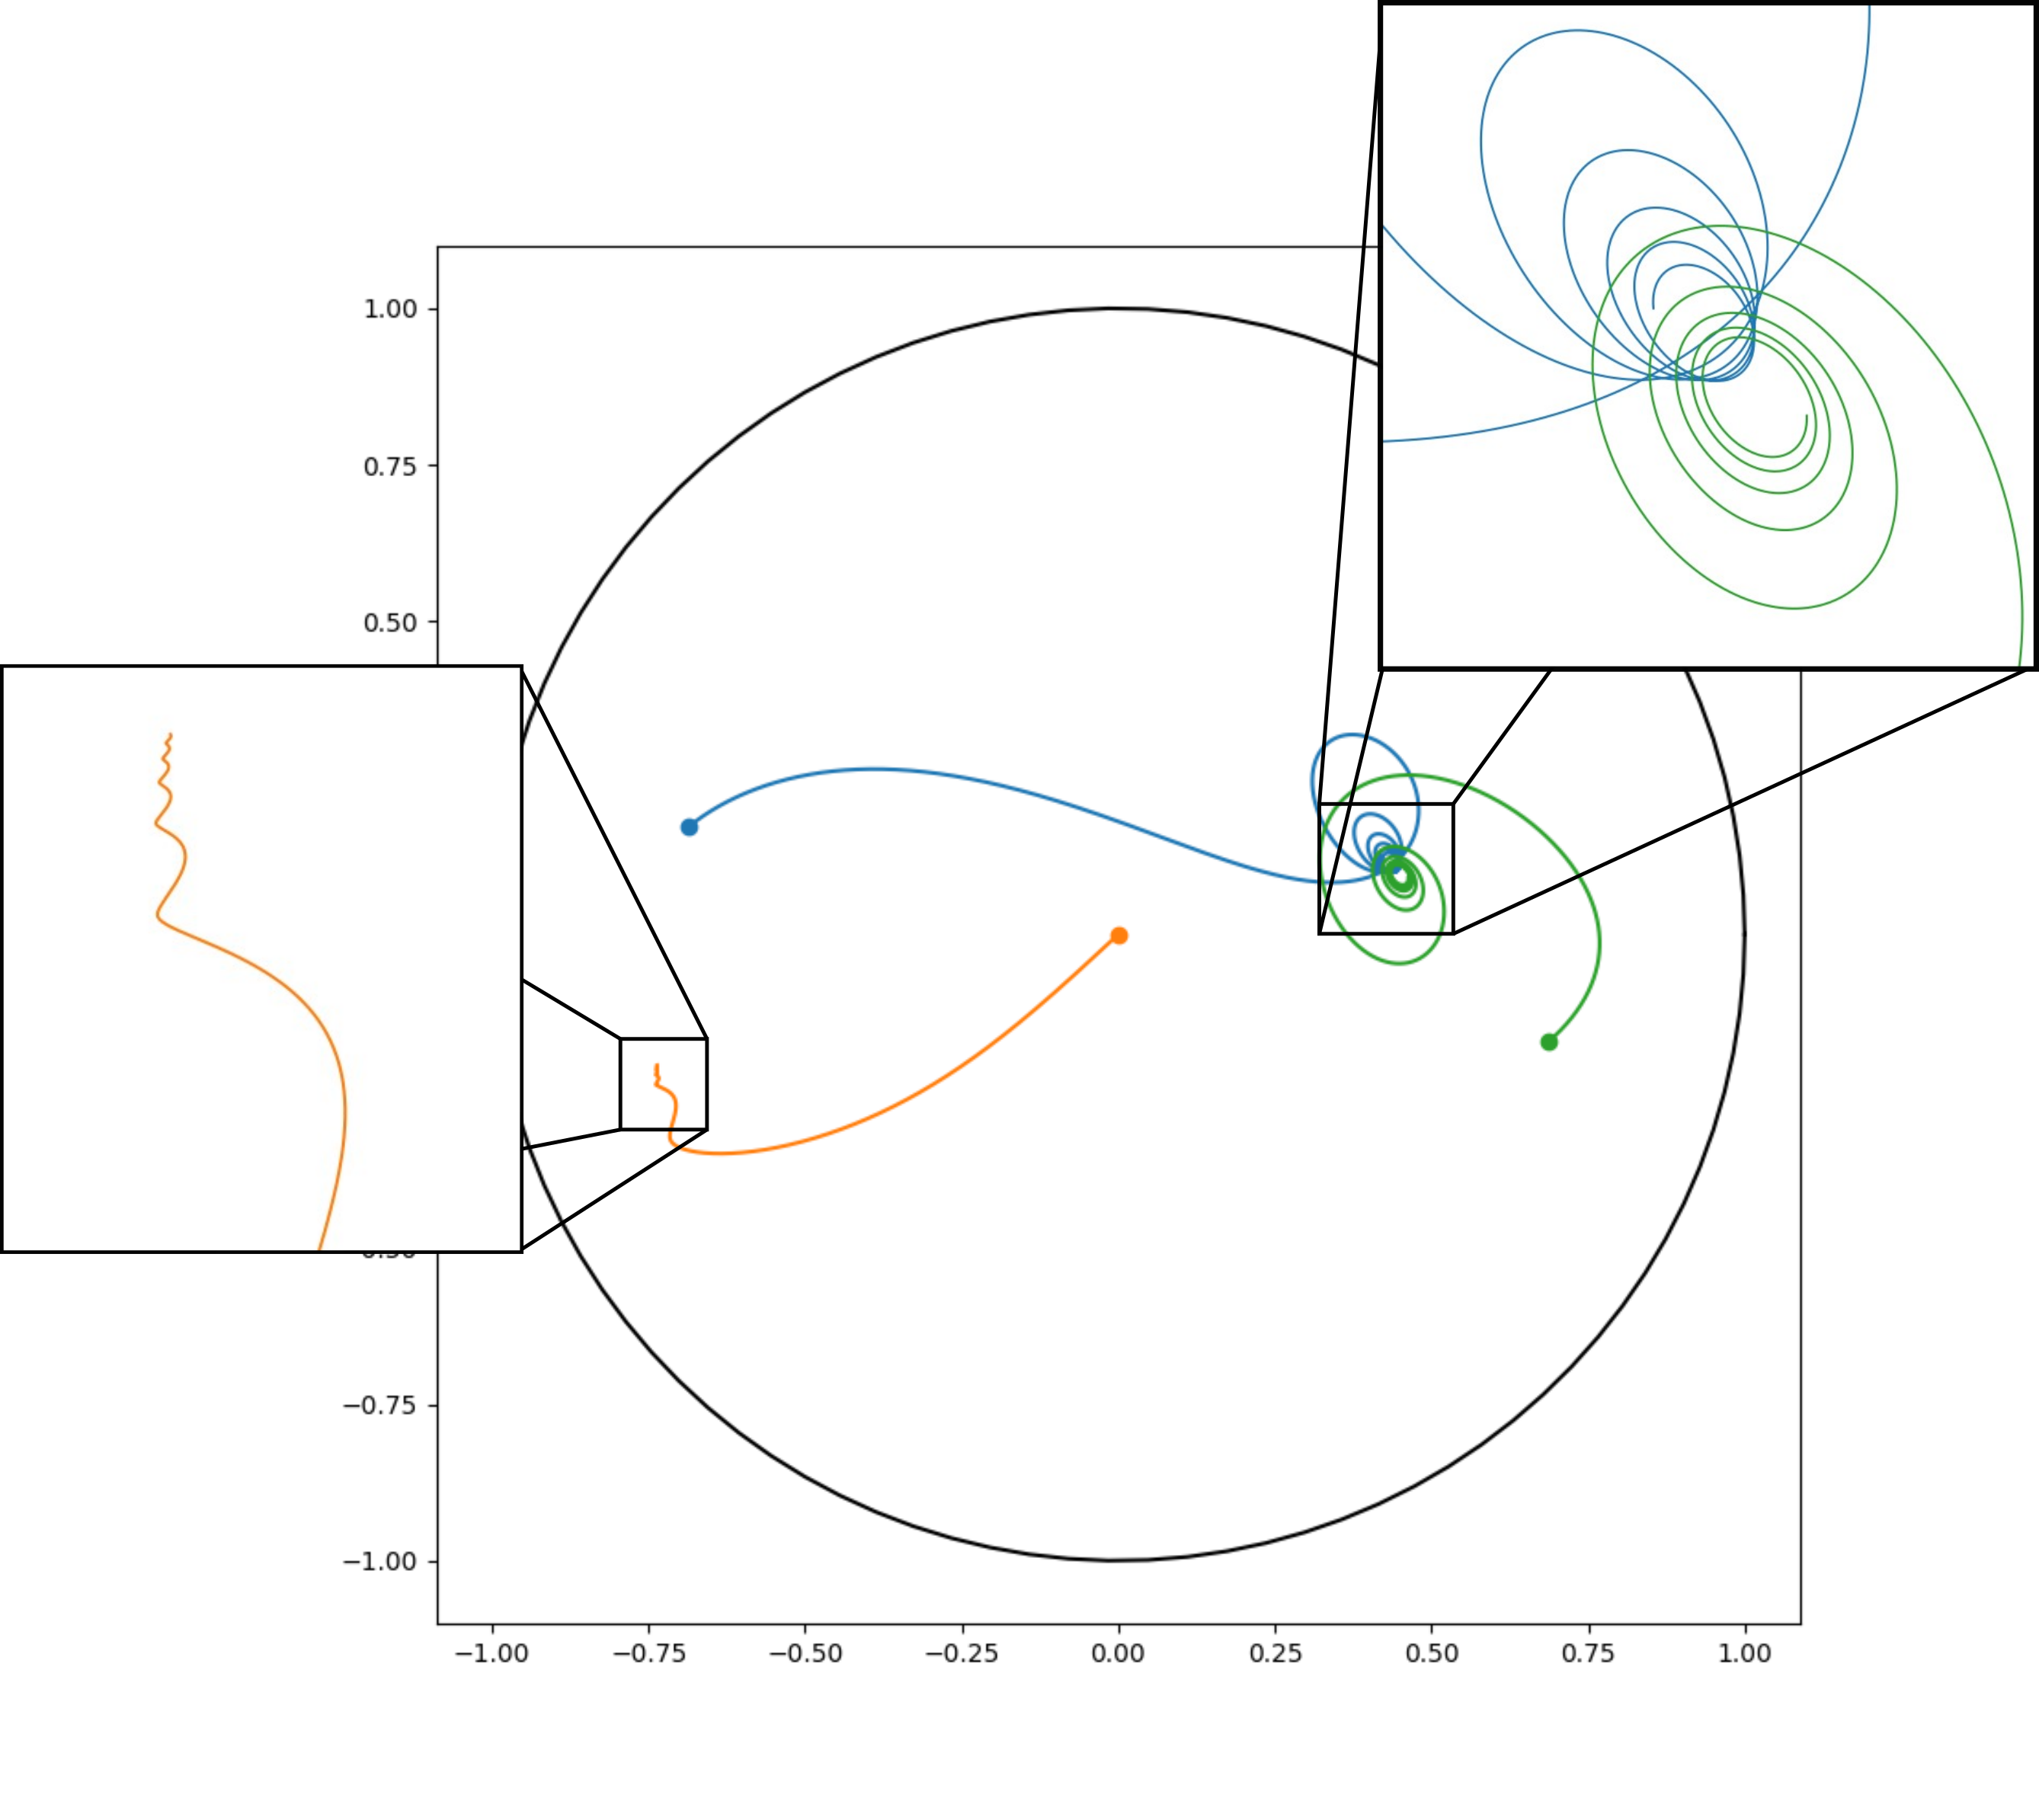
\includegraphics[width=\linewidth]{tcc//img/3corpos_energia0_posicoes_sd_zoom.png}
        \caption{Coordenadas de forma ($\vet \sigma$).}
        \label{fig:3corpos_energia0_posicoes_sd}
    \end{subfigure}%
    \begin{subfigure}{.5\textwidth}
        \centering
        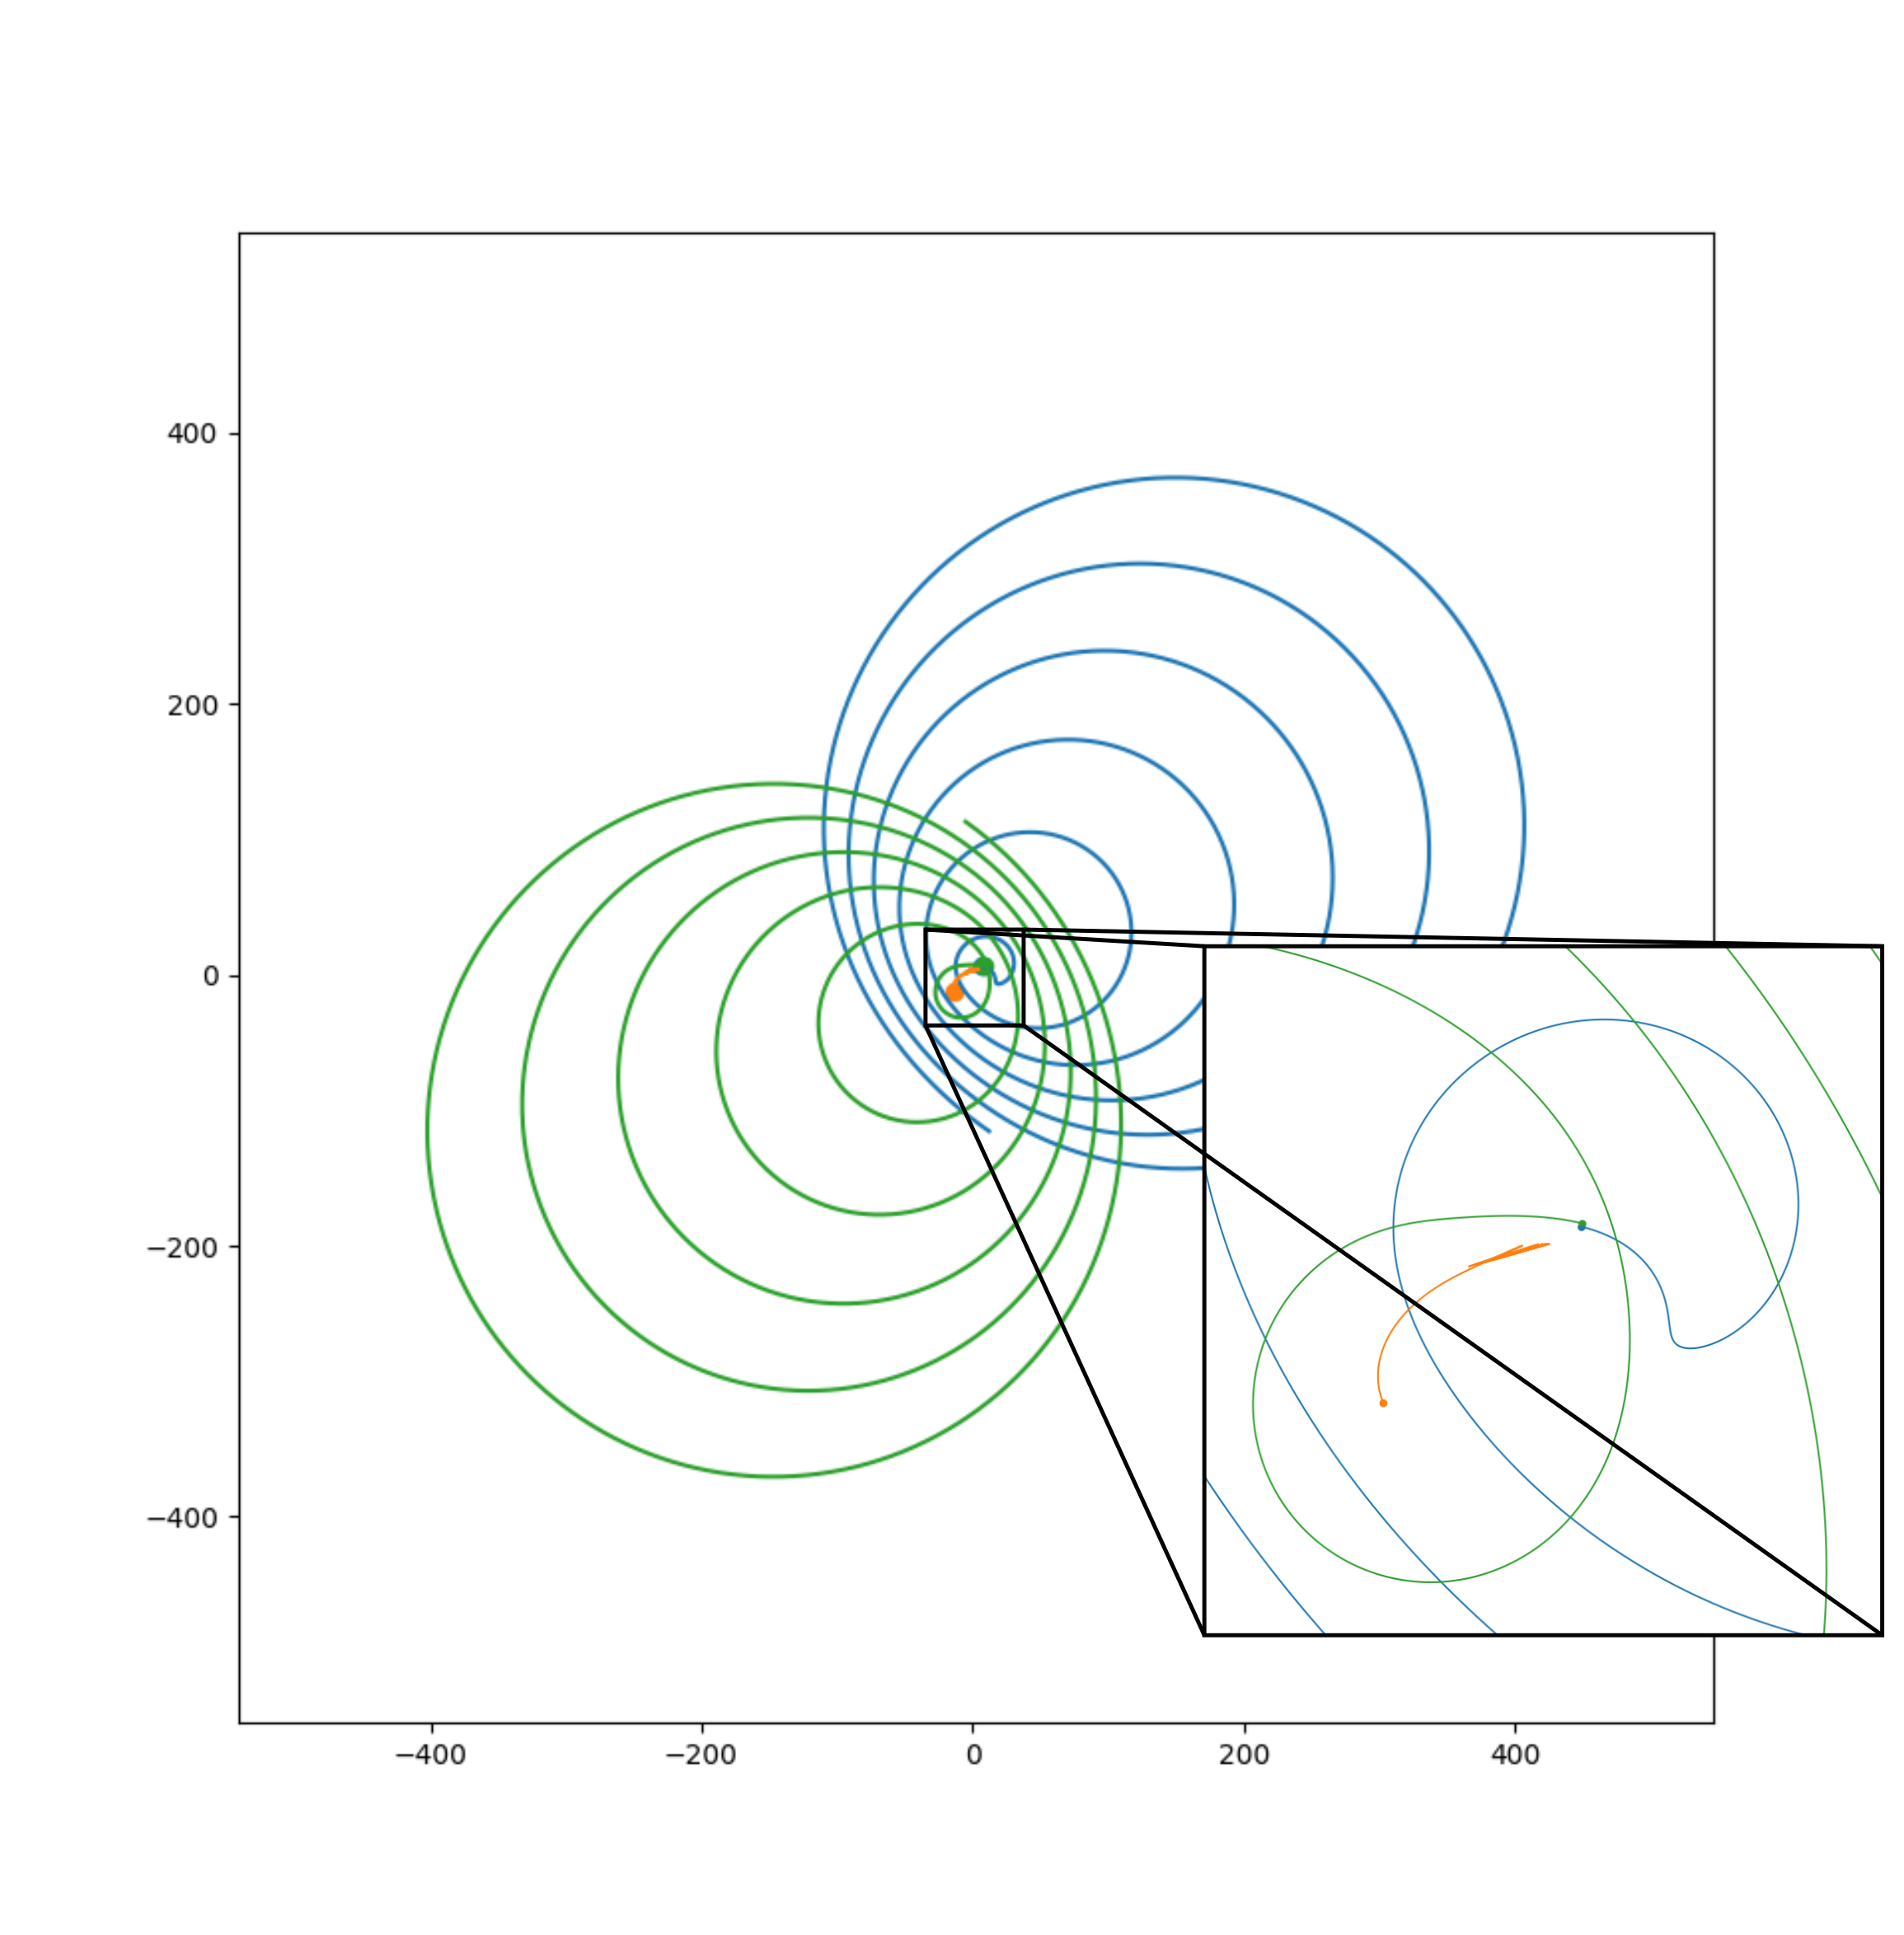
\includegraphics[width=\linewidth]{tcc//img/3corpos_energia0_velocidades_sd_zoom.png}
        \caption{Momentos de forma ($\vet \pi$).}
        \label{fig:3corpos_energia0_velocidades_sd}
    \end{subfigure}
    \caption{Coordenadas objetivas $(\vet \sigma, \vet \pi)$ do problema-modelo \ref{probmodelo:3corpos_energia_nula}.}
    \label{fig:probmodelo3corposenergia0_sd}
\end{figure}

Testamos também o comportamento de um sistema de 3 corpos com energia $E>0$, o problema-modelo \ref{probmodelo:3corpos_energia_positiva}, integrado no intervalo $[4.18,5000]$ via método SVCP8S15 com $h=10^{-4}$ sem correção. O motivo para o instante inicial específico é que o sistema começa com momento de dilatação negativo, e por facilidade foi fixado $h>0$, portanto no intervalo $[0,4.18)$ tem-se $D<0$, o que significa que o ponto de Janus para este caso está na vizinhança de $t=4.18$.

\begin{figure}[H]
    \centering
    \begin{subfigure}{.5\textwidth}
        \centering
        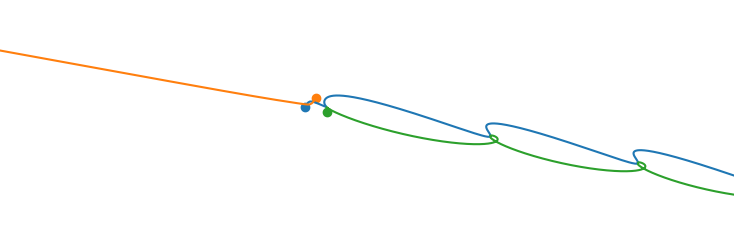
\includegraphics[width=0.8\linewidth]{tcc//img/3corpos_energiapositiva_posicoes_nd.png}
        \caption{}
        \label{fig:3corposenergiapositiva_trajetoria}
    \end{subfigure}%
    \begin{subfigure}{.5\textwidth}
        \centering
        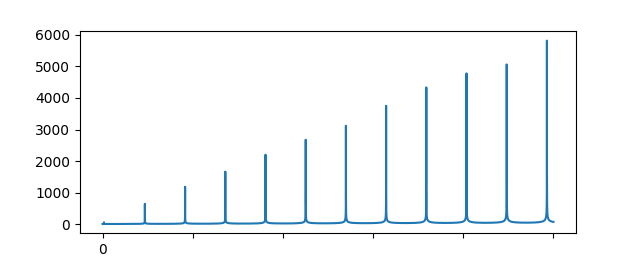
\includegraphics[width=\linewidth]{tcc//img/3corpos_energiapositiva_complexidade.png}
        \caption{}
        \label{fig:3corpos_energiapositiva_complexidade}
    \end{subfigure}
    
    \caption{Problema-modelo \ref{probmodelo:3corpos_energia_positiva}. À esquerda, recorte das trajetórias. À direita, a complexidade apresentada pelo sistema.}
    \label{fig:figuras_probmodel3_energia_positiva}
\end{figure}

Observe que neste problema os picos da complexidade são maiores (figura \ref{fig:3corpos_energiapositiva_complexidade}), refletindo a intensidade das aproximações do sistema binário formado. 

Isso se apresenta também nas coordenadas no espaço de formas. Como no problema com $E=0$, o corpo ejetado desacelera e começa a apresentar um comportamento cíclico e dissipativo (figura \ref{fig:3corpos_energiapositiva_posicoes_sd}). Porém, nesse caso a dissipação é bastante maior que no caso anterior. É visualmente notável a diferença na dissipação observando os momentos (figura \ref{fig:3corpos_energiapositiva_velocidades_sd}), pois o corpo dissipado tem momento oscilando próximo de zero e o sistema binário formado apresenta trajetórias circulares com raios cada vez maiores e com ordem de grandeza $10^5$, enquanto no caso $E=0$ tinha-se ordem de grandeza $10^2$.

\begin{figure}[H]
    \centering
    \begin{subfigure}{.5\textwidth}
        \centering
        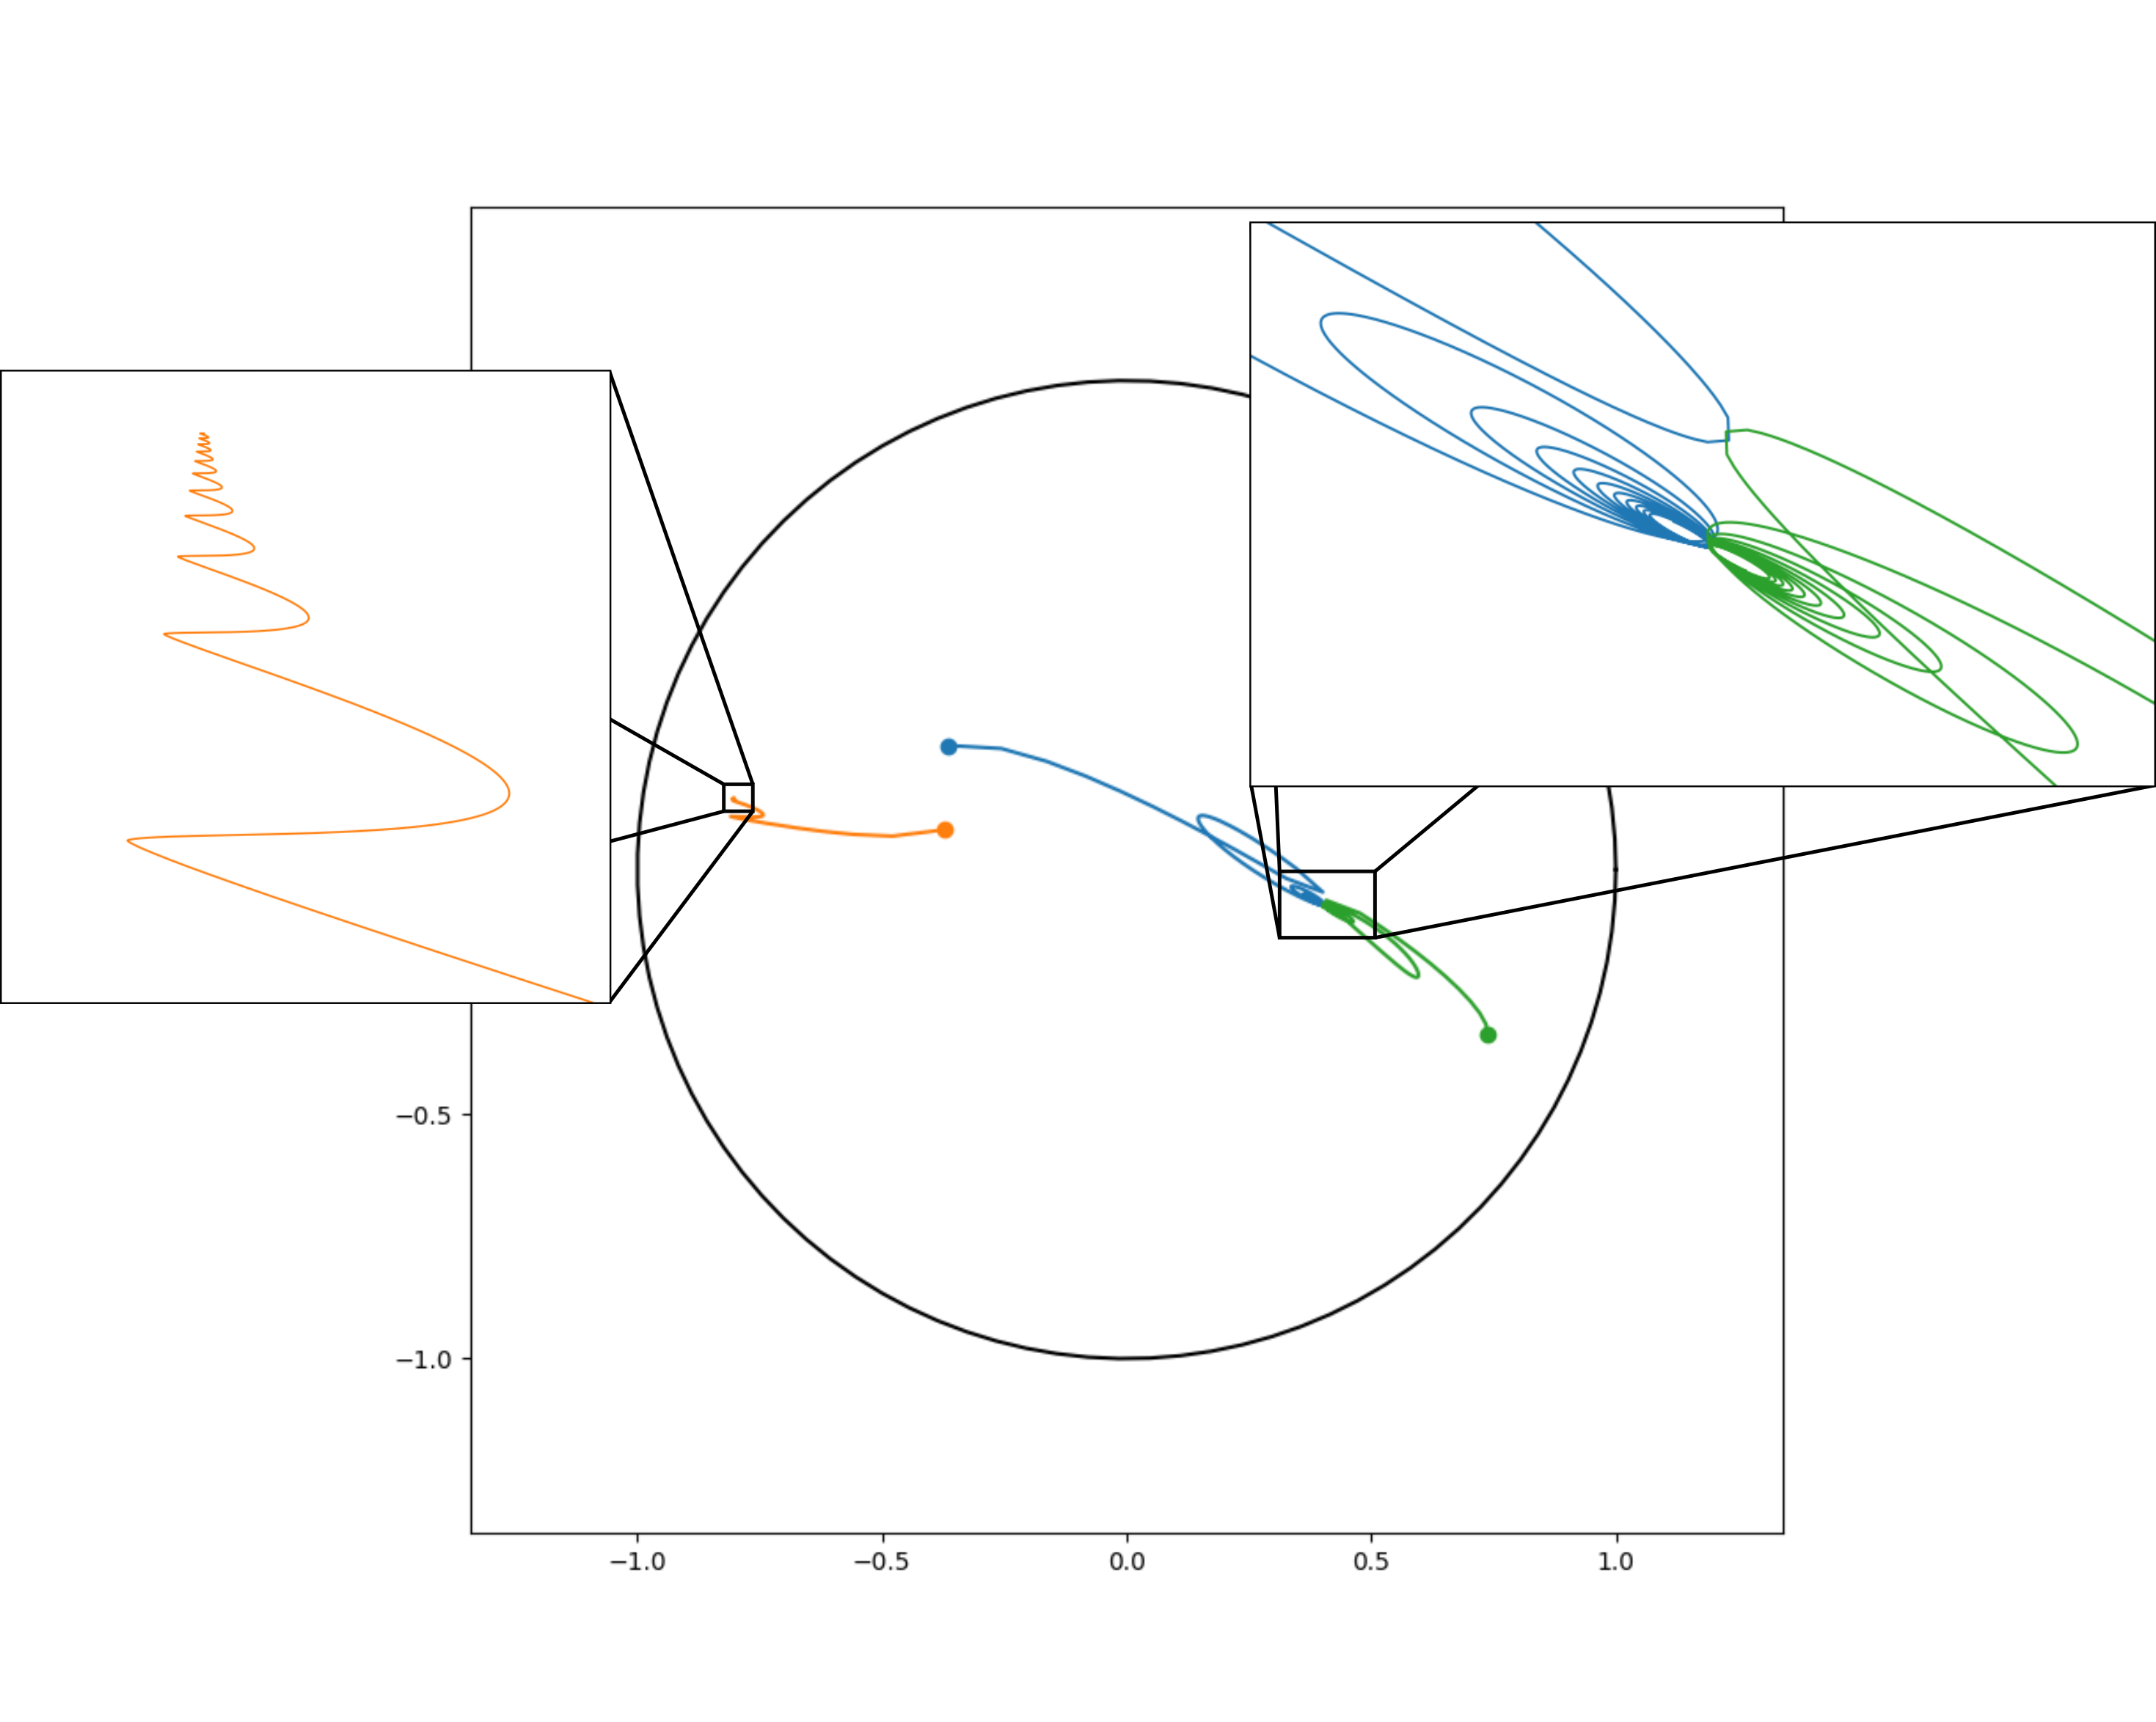
\includegraphics[width=\linewidth]{tcc//img/3corpos_energiapositiva_posicoes_sd_zoom.png}
        \caption{Coordenadas de forma ($\vet \sigma$).}
        \label{fig:3corpos_energiapositiva_posicoes_sd}
    \end{subfigure}%
    \begin{subfigure}{.5\textwidth}
        \centering
        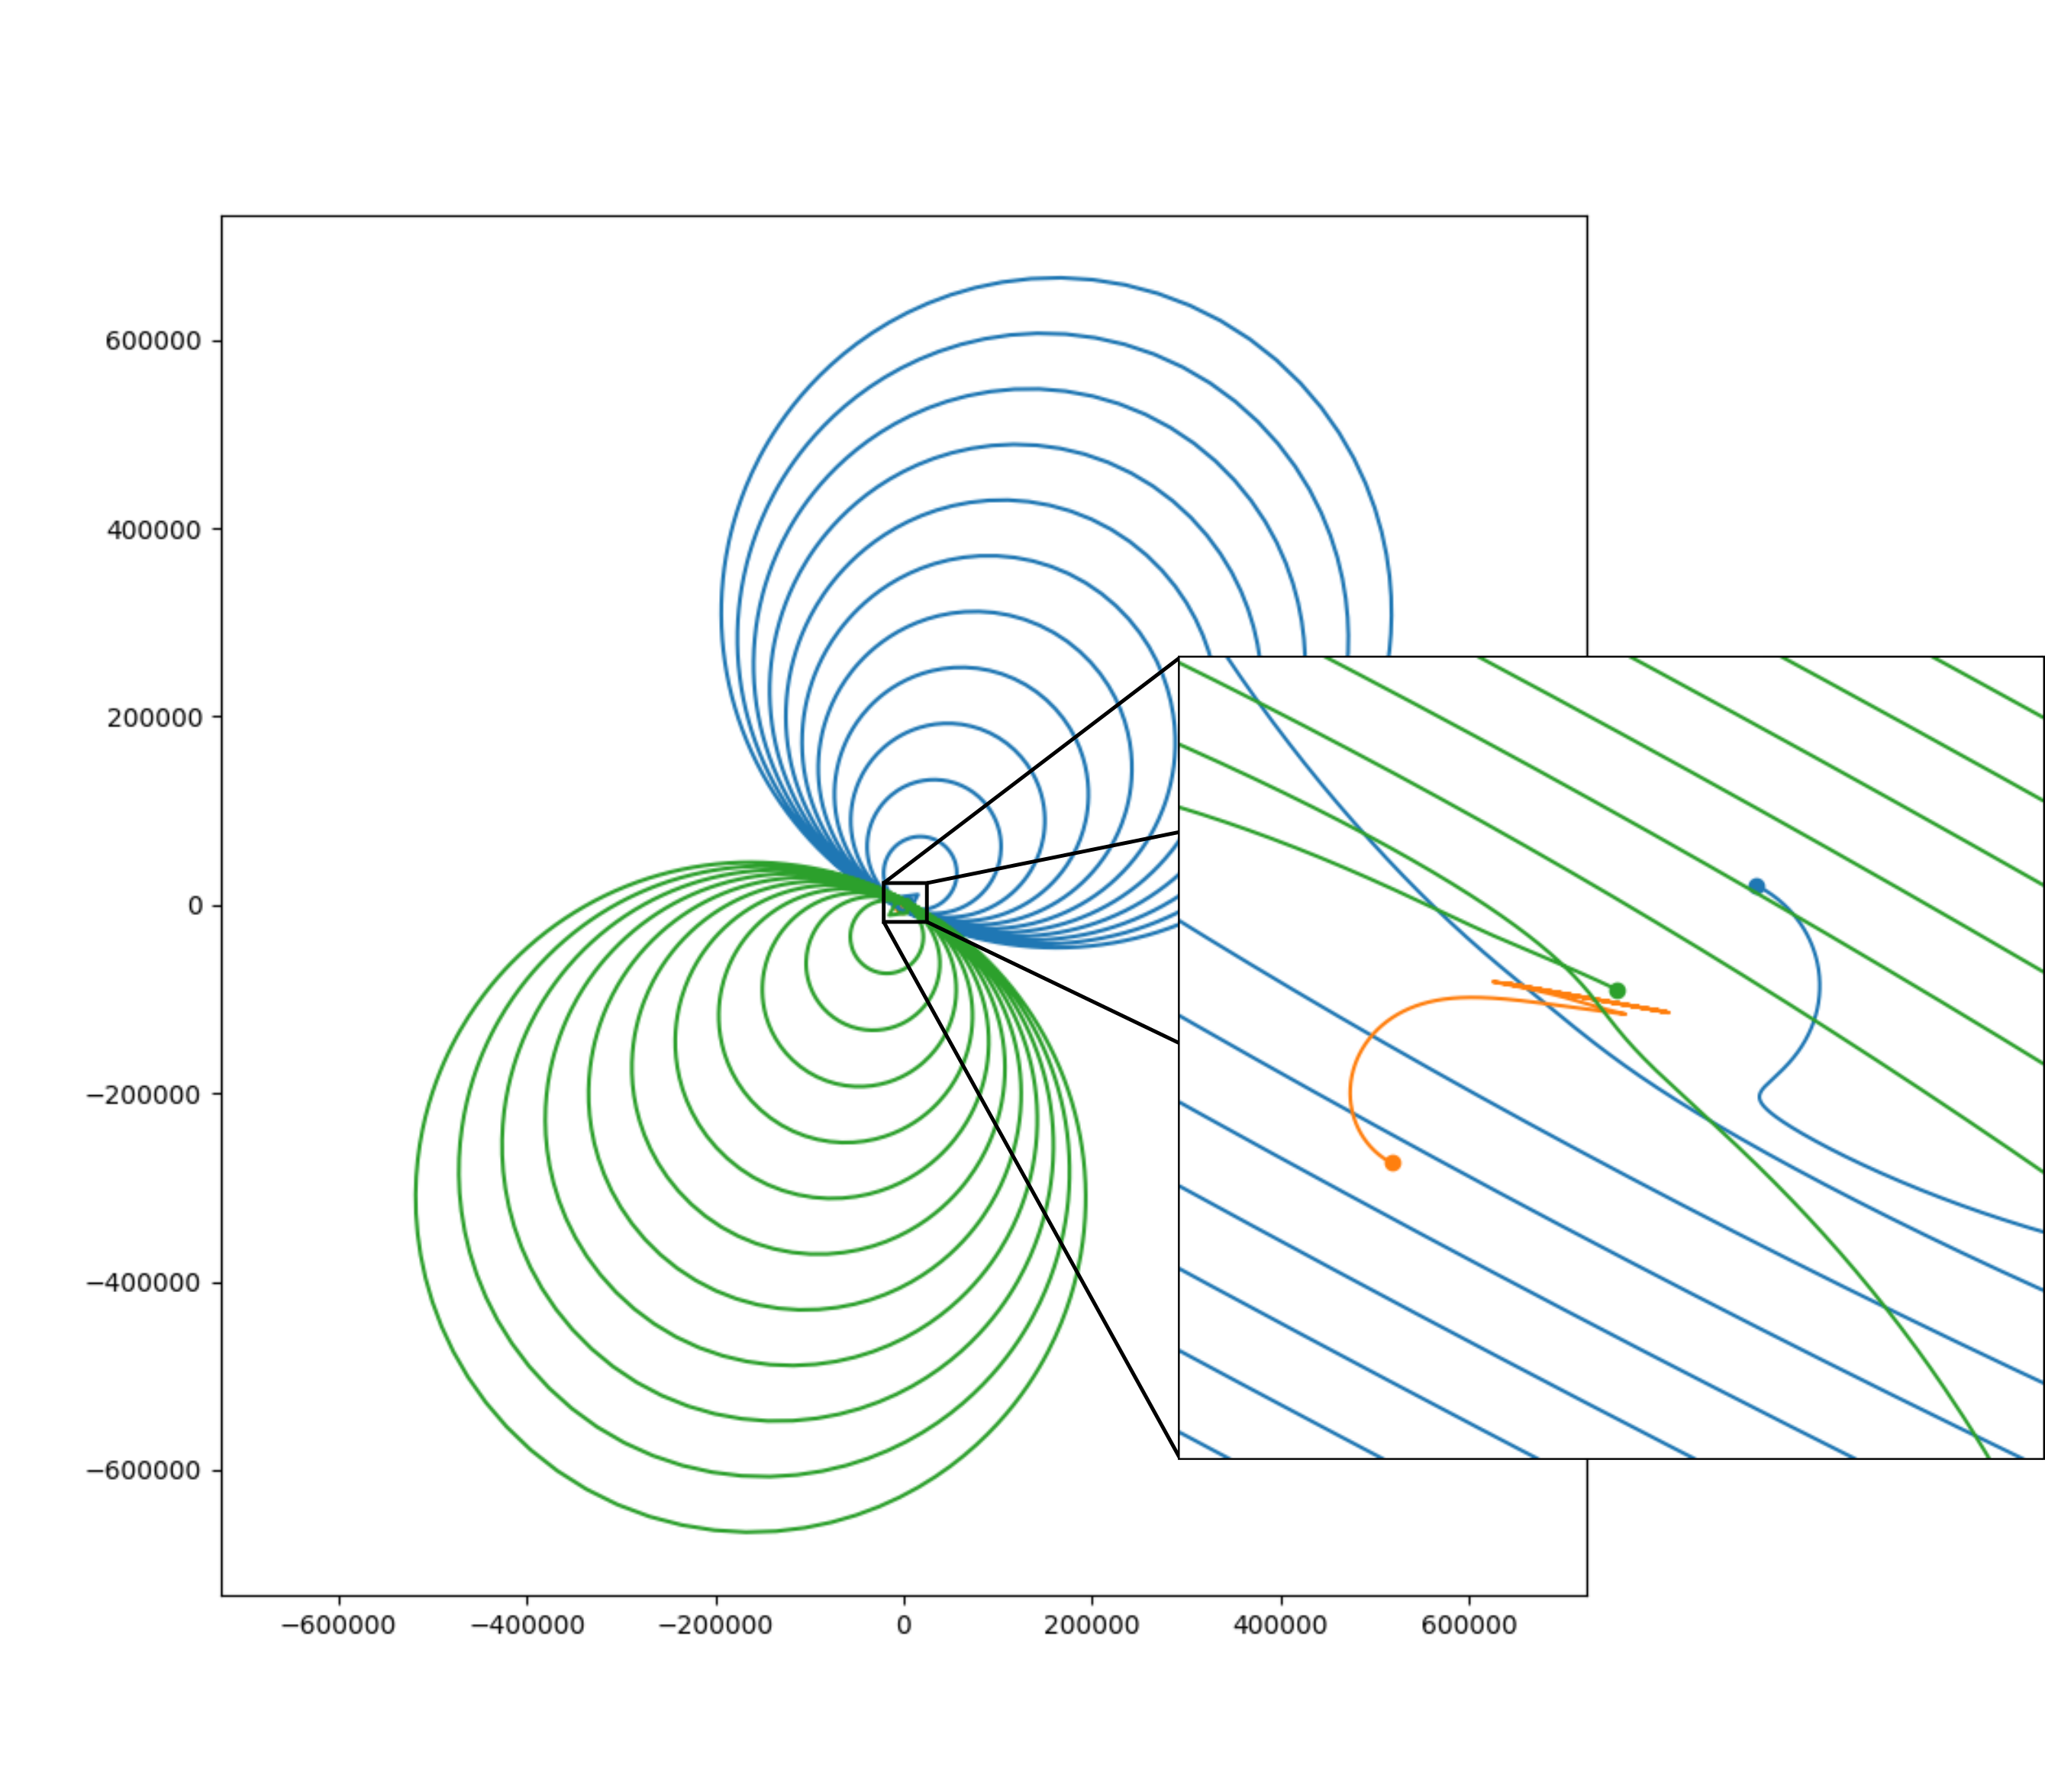
\includegraphics[width=\linewidth]{tcc//img/3corpos_energiapositiva_velocidades_sd_zoom.png}
        \caption{Momentos de forma ($\vet \pi$).}
        \label{fig:3corpos_energiapositiva_velocidades_sd}
    \end{subfigure}
    \caption{Coordenadas objetivas $(\vet \sigma, \vet \pi)$ do problema-modelo \ref{probmodelo:3corpos_energia_positiva}.}
    \label{fig:probmodelo3corposenergiapositiva_sd}
\end{figure}




%%%%%%%% PROBLEMA DE 20 CORPOS
\subsection{Problemas de 20 e 100 corpos}

Para problemas com $N \geq 10$, se mostrou pouco produtivo analisar as trajetórias no espaço de formas devido à quantidade de trajetórias. Além disso, dada a obrigatória separação do sistema em subsistemas em afastamento mútuo, a evolução no tempo newtoniano aumenta o momento de inércia $R^2$ mais rapidamente que o afastamento entre os corpos, levando as trajetórias no centro da esfera unitária a esferas cada vez menores e os corpos distantes a desacelerarem em algum ponto da esfera. 

\begin{figure}
    \centering
    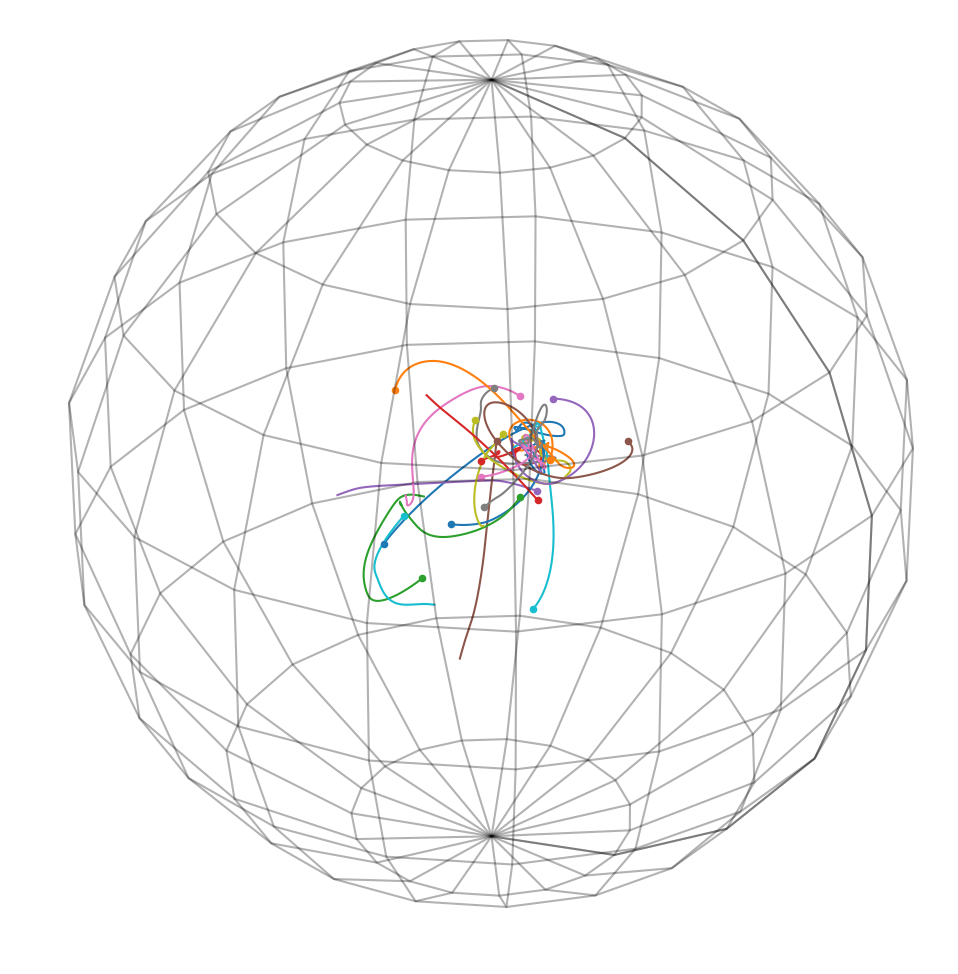
\includegraphics[width=0.5\linewidth]{tcc//img/20corpos_energia0_posicoes_3d_sd.png}
    \caption{Trajetória objetiva do problema-modelo \ref{probmodelo:20corpos_energia0}.}
    \label{fig:20corpos_trajetorias_sd}
\end{figure}

Para visualizar esse comportamento, simulamos o problema-modelo \ref{probmodelo:20corpos_energia0} com 20 corpos no intervalo $[0,5000]$ via RKN671 com $h=10^{-2}$ e $\epsilon=8h$. Nesse problema, todas as integrais primeiras são nulas. A trajetória objetiva pode ser visualizada na figura \ref{fig:20corpos_trajetorias_sd}.

A complexidade (figura \ref{fig:20corpos_complexidade}), porém, para $N=20$ já apresenta mais nitidamente o comportamento esperado: a expansão do sistema (grande escala) faz com que $C_S$ cresça no tempo newtoniano, e as interações entre os subsistemas (pequena escala) se apresentam nas variações desse crescimento, bastante nítidas nos casos de aproximações intensas facilmente identificáveis pelos maiores picos de $C_S$.

\begin{figure}[H]
    \centering
    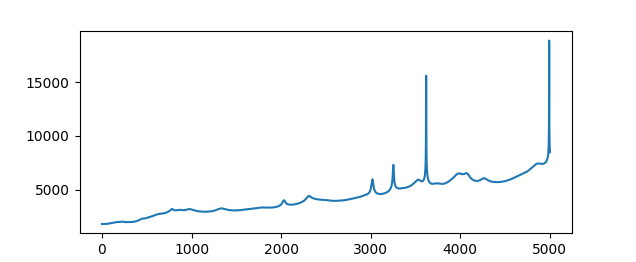
\includegraphics[width=0.8\linewidth]{tcc//img/20corpos_energia0_complexidade.png}
    \caption{Complexidade do problema-modelo \ref{probmodelo:20corpos_energia0}.}
    \label{fig:20corpos_complexidade}
\end{figure}

Simulamos também um problema de 100 corpos com todas as integrais primeiras nulas (\ref{probmodelo:100corpos_energia0}) no intervalo $[-10^6,10^6]$ via método de Verlet com $h=0.04=\epsilon$ em paralelo. Vale ressaltar que a simulação levou cerca de 108 segundos.

Na figura \ref{fig:100corpos_complexidade} podemos observar como as propriedades da complexidade se mostram ainda mais nítidas que no caso $N=20$. Além disso, como foi feita também a integração para o passado, é possível visualizar o ponto de Janus (o mínimo de $C_S$). Nesse caso, dada a grande variação de $C_S$, é possível observar que o sistema não apresentou grande expansão num primeiro momento, mas uma quantidade grande de interações no centro de massas.

\begin{figure}
    \centering
    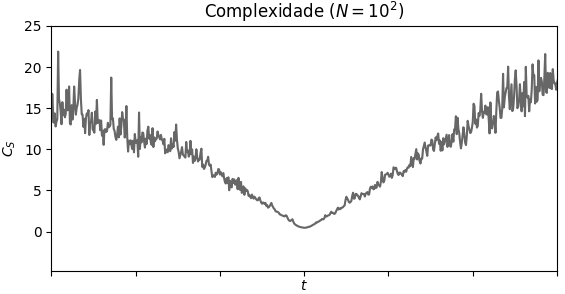
\includegraphics[width=0.6\linewidth]{tcc//img/complexidade100.png}
    \caption{Complexidade do problema-modelo \ref{probmodelo:100corpos_energia0}.}
    \label{fig:100corpos_complexidade}
\end{figure}


%%%%%%%% PROBLEMA DE 1000 CORPOS
\subsection{Problemas de 1000 corpos}

Passando para escalas maiores, realizamos três simulações com $N=10^3$ no intervalo $[-10^4, 10^4]$ via método de Verlet com $h=0.04=\epsilon=h$ para observar o comportamento de $C_S$ com diferentes valores de $E$: $-0.25$, $0$ e $0.25$.


\subsubsection{Energia total nula}

Começando pelos casos nos quais temos informações esperadas sobre o comportamento, o problema-modelo \ref{probmodelo:1000corpos_energianula} contém as condições iniciais para $E=0$ (todas as integrais primeiras são nulas, na verdade). Na figura \ref{fig:1000corpos_energia0_complexidade} é possível observar o crescimento variado de $C_S$ de maneira semelhante em relação ao eixo definido pelo Ponto de Janus. A vizinhança desse instante se apresentou nesse caso como um momento de rápida expansão e intensas aproximações, seguido pelo início de um momento de maior estabilidade tanto dos corpos ejetados quanto dos corpos ainda próximos ao centro. 

\begin{figure}[H]
    \centering
    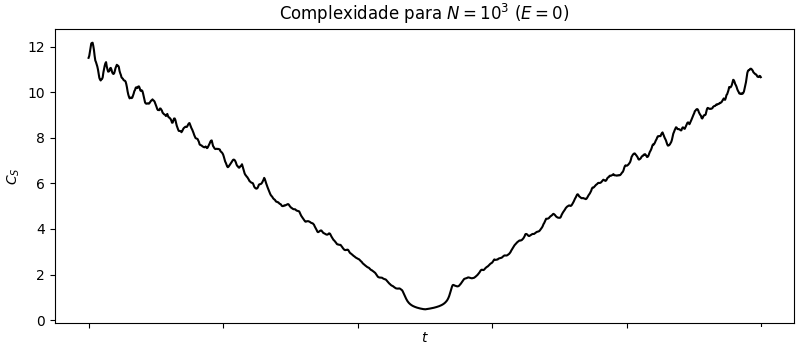
\includegraphics[width=0.6\linewidth]{tcc//img/complexidade_1000_nula.png}
    \caption{Complexidade do problema-modelo \ref{probmodelo:1000corpos_energianula}.}
    \label{fig:1000corpos_energia0_complexidade}
\end{figure}

A evolução do sistema pode ser observada na figura \ref{fig:1000corpos_energia0_posicoes}. O centro de massas concentra grande parte dos corpos mesmo nos limites do intervalo considerado, mas a ejeção de partículas continua acontecendo.

\begin{figure}[H]
    \centering
    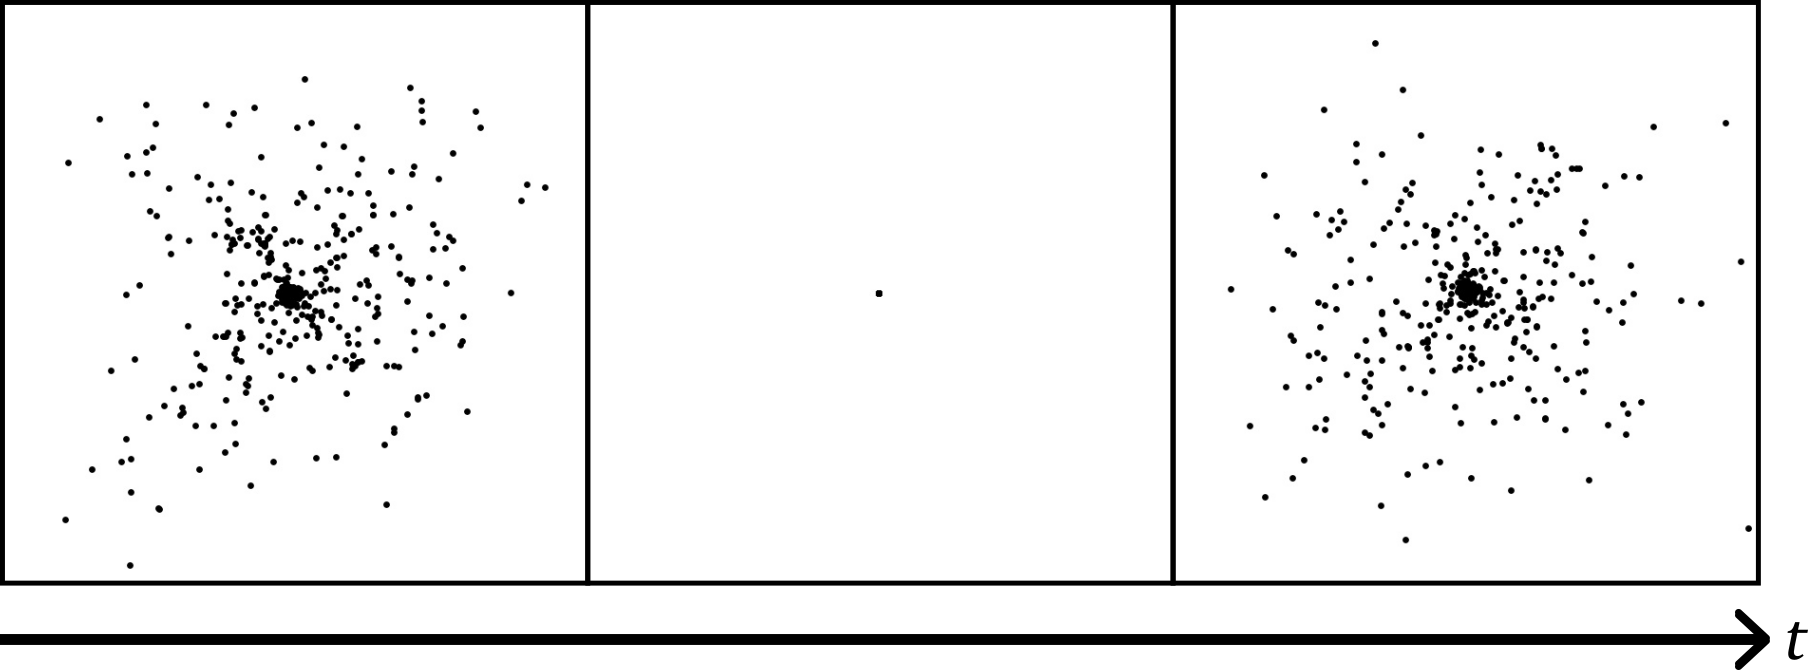
\includegraphics[width=0.8\linewidth]{tcc//img/espalhamento_energia_nula_1000.png}
    \caption{Instantes do bordo e $t=0$ do problema-modelo \ref{probmodelo:1000corpos_energianula}.}
    \label{fig:1000corpos_energia0_posicoes}
\end{figure}


\subsubsection{Energia total positiva}
Já para o caso $E=0.25$ no problema-modelo \ref{probmodelo:1000corpos_energiapositiva_1}, com massas $m=1/N$, observamos uma baixa variação de $C_S$ (figura \ref{fig:1000corpos_energiapositiva_complexidade_1}). Como o sistema necessariamente se contrai e se expande (devido ao comportamento do momento de inércia previsto pela relação de Lagrange-Jacobi), isso indica que a interação gravitacional entre os corpos é quase inversamente proporcional ao tamanho do sistema, o que sugere a não formação de binários e, do ponto de vista da do espaço de formas, o resultado é o esperado: o sistema assintoticamente congela.

\begin{figure}[H]
    \centering
    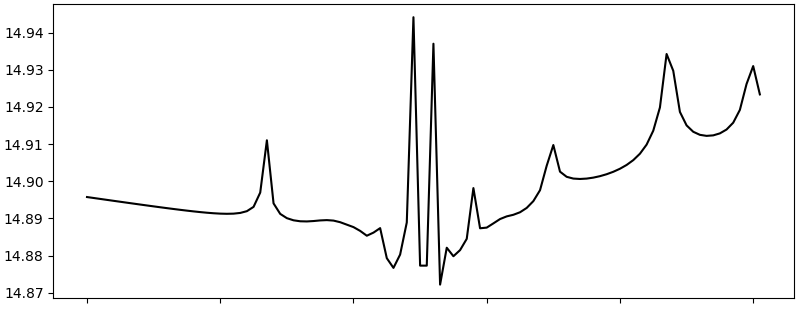
\includegraphics[width=0.6\linewidth]{tcc//img/1000corpos_energiapositiva_complexidade_1.png}
    \caption{Complexidade do problema-modelo \ref{probmodelo:1000corpos_energiapositiva_1}.}
    \label{fig:1000corpos_energiapositiva_complexidade_1}
\end{figure}

Na figura \ref{fig:1000corpos_energiapositiva_posicoes_1} é possível observar um espalhamento bastante uniforme dos corpos no espaço. Uma vez que os valores iniciais foram gerados através de uma distribuição uniforme, isso reflete o baixo nível de interação entre os corpos.

\begin{figure}[H]
    \centering
    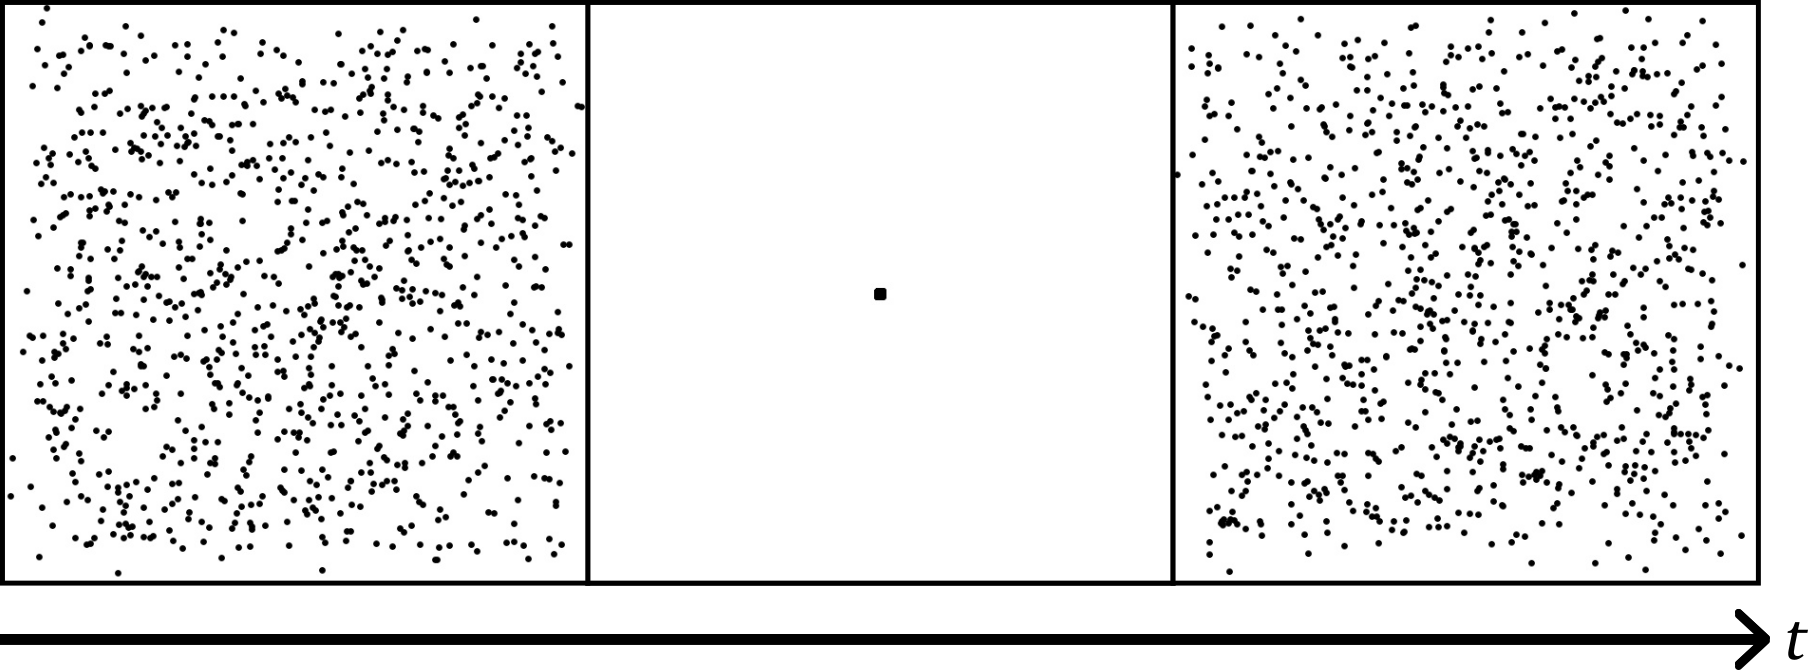
\includegraphics[width=0.8\linewidth]{tcc//img/espalhamento_energia_positiva_1000.png}
    \caption{Instantes do bordo e $t=0$ do problema-modelo \ref{probmodelo:1000corpos_energiapositiva_1}.}
    \label{fig:1000corpos_energiapositiva_posicoes_1}
\end{figure}


Optamos então por gerar novos valores iniciais mas com massas um pouco maiores individualmente, mas o suficiente para o sistema aumentar $10^3$ vezes em massa total (problema-modelo \ref{probmodelo:1000corpos_energiapositiva_2}). Nesse caso, o problema apresentou um comportamento mais parecido com o caso $E=0$, pois as interações gravitacionais foram mais intensas (veja figura \ref{fig:1000corpos_energiapositiva_posicoes_2}).

\begin{figure}[H]
    \centering
    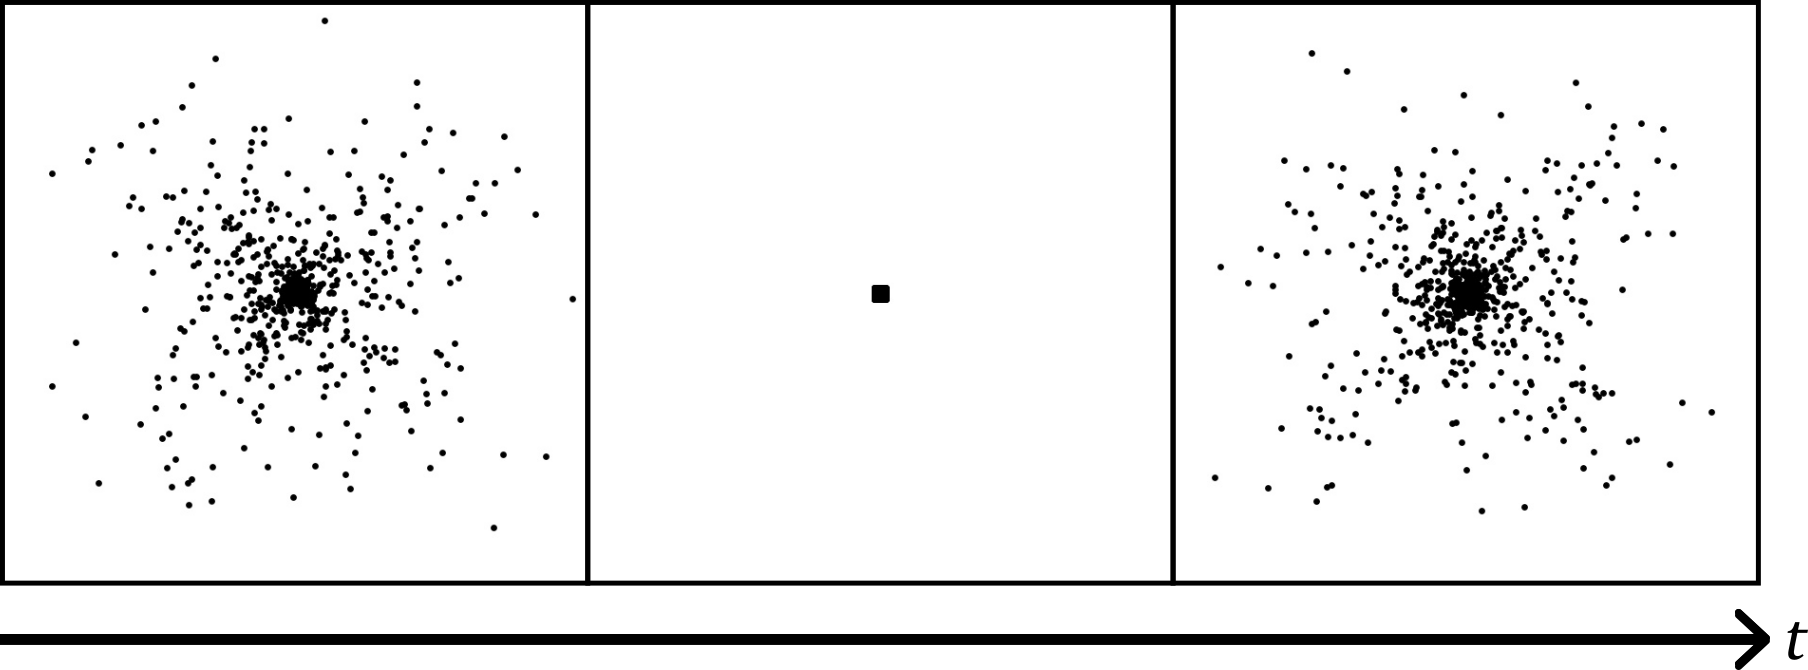
\includegraphics[width=0.8\linewidth]{tcc//img/espalhamento_energia_positiva_1000_2.png}
    \caption{Instantes do bordo e $t=0$ do problema-modelo \ref{probmodelo:1000corpos_energiapositiva_2}.}
    \label{fig:1000corpos_energiapositiva_posicoes_2}
\end{figure}

A complexidade também apresentou um comportamento diferente do primeiro exemplo de $E=0.25$ com um formato semelhante ao de $E=0$, mas com uma grande diferença de escala (veja figura \ref{fig:1000corpos_energiapositiva_complexidade_2}).

\begin{figure}
    \centering
    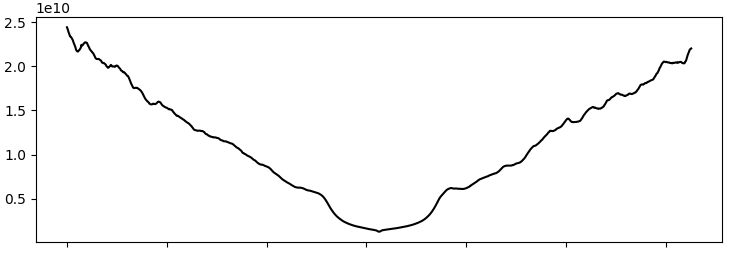
\includegraphics[width=0.8\linewidth]{tcc//img/1000corpos_energiapositiva_complexidade_2.png}
    \caption{Complexidade no problema-modelo \ref{probmodelo:1000corpos_energiapositiva_2}.}
    \label{fig:1000corpos_energiapositiva_complexidade_2}
\end{figure}


\subsubsection{Energia total negativa}
Por fim, no caso $E=-0.25$ tivemos um resultado curioso. Embora as condições impostas inicialmente tenham sido as de Hénon (veja subseção \ref{subsection:condicoes_aarseth}), a complexidade apresentou um comportamento de cúspide (figura \ref{fig:1000corpos_energianegativa_complexidade}. O que ocorre é que na evolução do sistema nesse caso são ejetados alguns corpos (o que provoca o crescimento) mas mantém relativa estabilidade no centro de massas.

\begin{figure}[H]
    \centering
    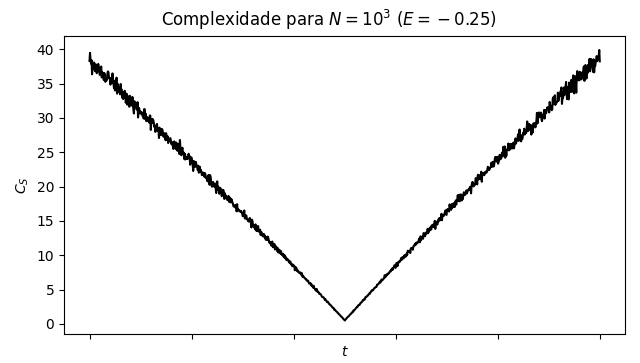
\includegraphics[width=0.6\linewidth]{tcc//img/complexidade1000_energianegativa.png}
    \caption{Complexidade no problema-modelo \ref{probmodelo:1000corpos_energianegativa}.}
    \label{fig:1000corpos_energianegativa_complexidade}
\end{figure}

Esse comportamento pode ser observado na figura \ref{fig:1000corpos_energianegativa_posicoes}, onde a maior parte do sistema fica contida na região central enquanto alguns poucos corpos são ejetados, sem formação de binários.

\begin{figure}[H]
    \centering
    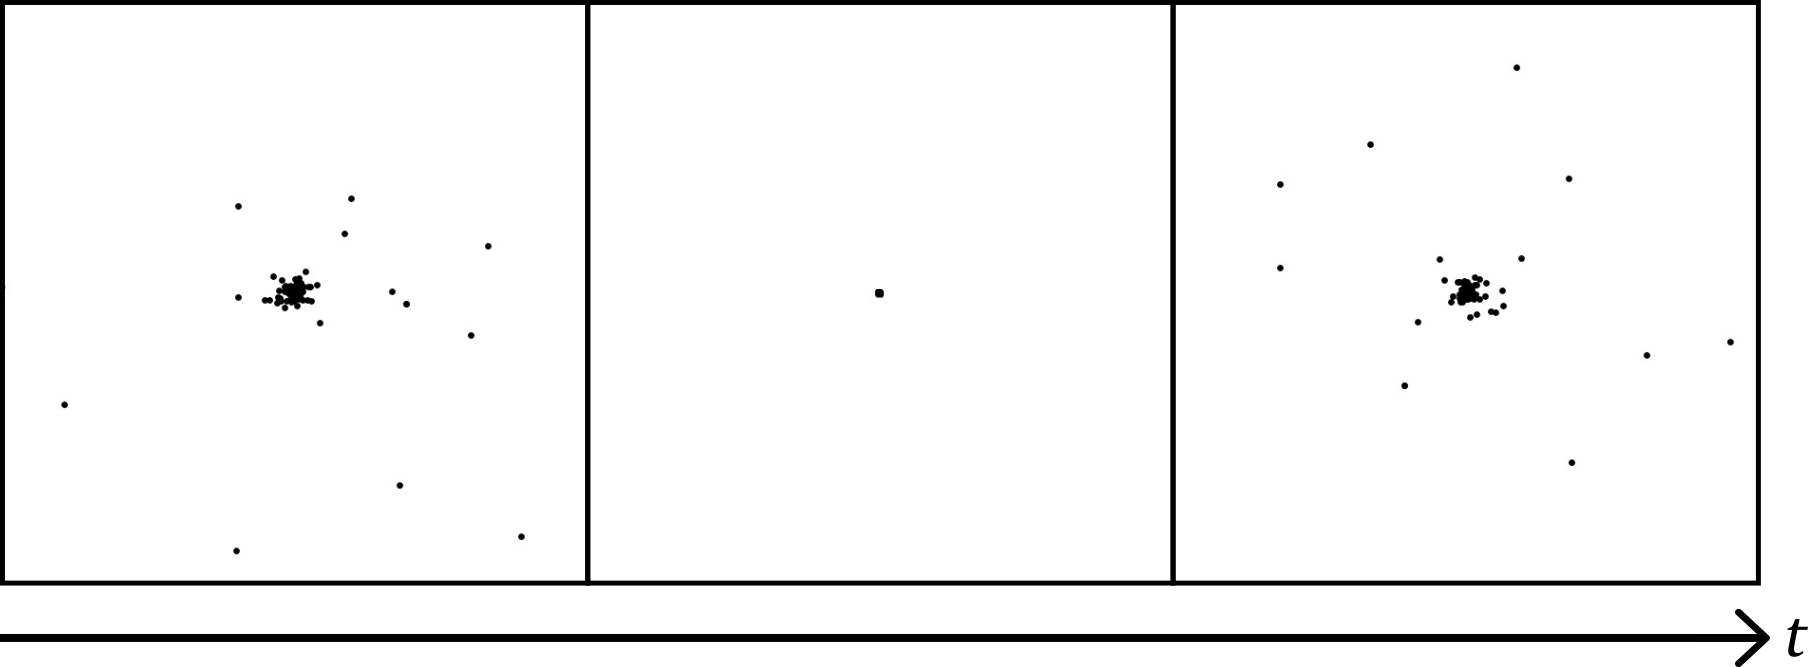
\includegraphics[width=0.8\linewidth]{tcc//img/espalhamento_energia_negativa_1000.png}
    \caption{Instantes do bordo e $t=0$ do problema-modelo \ref{probmodelo:1000corpos_energianegativa}.}
    \label{fig:1000corpos_energianegativa_posicoes}
\end{figure}

Na vizinhança do Ponto de Janus, porém, é possível encontrar semelhanças com os casos $E \geq 0$, como na formação de um pequeno ``vale'' a princípio seguido do início da variação (figura \ref{fig:1000corpos_energianegativa_complexidade_zoom}).

\begin{figure}[H]
    \centering
    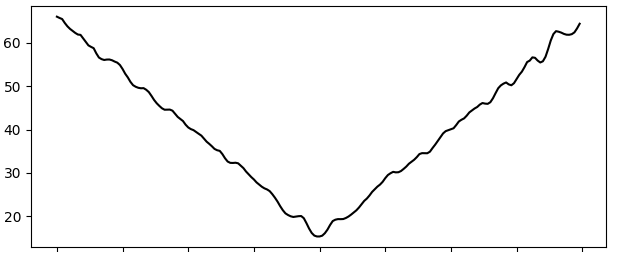
\includegraphics[width=0.8\linewidth]{tcc/img/zoom_complexidade_1000corpos_negativa.png}
    \caption{Vizinhança do ponto de Janus no problema $N=10^3$ com $E=-0.25$.}
    \label{fig:1000corpos_energianegativa_complexidade_zoom}
\end{figure}

% * TESTES PRATICOS E PROGRAMA FINAL
%    
%   Fazer alguns testes legais e apresentar como o programa 
%   ficou no final.
%   ????